\documentclass[12pt]{article}
\usepackage[margin=1in]{geometry}
\usepackage{booktabs}
\usepackage{longtable}
\usepackage{caption}
\usepackage{graphicx}
\usepackage{float}
\usepackage{array}
\usepackage{lscape}
\DeclareCaptionLabelSeparator{emdash}{---}
\captionsetup{font=normalsize,labelfont=sc,textfont=sc,labelsep=emdash}
\captionsetup[figure]{position=top,justification=centering}
\def\sym#1{\ifmmode^{#1}\else\(^{#1}\)\fi}
\graphicspath{{../Output/Figures/Main/}{../Output/Figures/Appendix/}{../Output/Figures/Online_Appendix/}{./}}
\title{Results First Draft}
\author{Zachary Serby}
\date{\today}
\begin{document}
\maketitle
\thispagestyle{empty}
\clearpage

\section*{Main}
\subsection*{Summary Statistics}

\begingroup
\footnotesize
\renewcommand{\arraystretch}{0.86}
\setlength{\tabcolsep}{4pt}
\setlength{\LTcapwidth}{\textwidth}
\begin{longtable}{l*{6}{c}}
\caption{Summary Statistics, Discrete-Dose Samples}\\
\toprule
 & \multicolumn{6}{c}{Panel A: WAZ, age \ensuremath{\le}10 in 2005 and 2009}\\
\cmidrule(lr){2-7}
                    &        Mean&   Std. dev.&        Min.&      Median&        Max.&        Obs.\\
\midrule
\textit{Outcomes (MxFLS-2, 2005)}&            &            &            &            &            &            \\
Weight-for-age z-score (WAZ)&       -0.30&        1.42&       -5.07&       -0.36&        4.51&       1,045\\
\addlinespace[6pt]\textit{Outcome change, 2005 to 2009}&            &            &            &            &            &            \\
Change in WAZ       &        0.55&        1.41&       -4.88&        0.46&        9.10&       1,045\\
\addlinespace[6pt]\textit{Dose levels (CHIRPS)}&            &            &            &            &            &            \\
2009 rainfall, z    &       -0.50&        0.83&       -2.24&       -0.39&        0.96&       1,045\\
Near normal, \ensuremath{-1<z<1}&        0.65&        0.48&        0.00&        1.00&        1.00&       1,045\\
Moderately dry, \ensuremath{-1.5<z\le -1}&        0.21&        0.41&        0.00&        0.00&        1.00&       1,045\\
Severely dry or worse, \ensuremath{z\le -1.5}&        0.14&        0.35&        0.00&        0.00&        1.00&       1,045\\

\bottomrule
\addlinespace[12pt]
\toprule
 & \multicolumn{6}{c}{Panel B: HAZ and BMIZ, age \ensuremath{\le}15 in 2005 and 2009}\\
\cmidrule(lr){2-7}
                    &        Mean&   Std. dev.&        Min.&      Median&        Max.&        Obs.\\
\midrule
\textit{Outcomes (MxFLS-2, 2005)}&            &            &            &            &            &            \\
Height-for-age z-score (HAZ)&       -0.58&        1.49&       -5.46&       -0.63&        5.65&       2,351\\
BMI-for-age z-score (BMIZ)&        0.36&        1.43&       -4.95&        0.30&        4.86&       2,310\\
\addlinespace[6pt]\textit{Outcome change, 2005 to 2009}&            &            &            &            &            &            \\
Change in HAZ       &        0.07&        1.37&       -5.93&        0.07&        6.35&       2,351\\
Change in BMIZ      &        0.23&        1.31&       -5.90&        0.17&        7.59&       2,295\\
\addlinespace[6pt]\textit{Dose levels (CHIRPS)}&            &            &            &            &            &            \\
2009 rainfall, z    &       -0.55&        0.84&       -2.24&       -0.53&        0.96&       2,351\\
Near normal, \ensuremath{-1<z<1}&        0.64&        0.48&        0.00&        1.00&        1.00&       2,351\\
Moderately dry, \ensuremath{-1.5<z\le -1}&        0.21&        0.41&        0.00&        0.00&        1.00&       2,351\\
Severely dry or worse, \ensuremath{z\le -1.5}&        0.16&        0.36&        0.00&        0.00&        1.00&       2,351\\

\bottomrule
\addlinespace[6pt]\multicolumn{7}{p{0.97\textwidth}}{\scriptsize \textit{Notes:} This table is for the discrete-dose specification, the main model. Obs. counts children. The sample is children with the outcome measured in MxFLS-2 (2005) and MxFLS-3 (2009), under the panel's age cutoff
in both survey waves, with a 2005 municipality. They were not measured in MxFLS-3 before November 2009. I use November 2009 as the cutoff because the 2009 rainfall deficit had not fully occurred before then. Dropping them from both groups equalizes treated and control measurement timing. Children in wet municipalities (z of 1 or above) are excluded.
Panel A uses the WAZ sample, Panel B the HAZ and BMIZ sample. The BMIZ sample is marginally smaller than the HAZ sample shown in Panel B, at 2,300 children. Statistics are at the 2005 baseline, except the change in WAZ, HAZ and BMIZ from 2005 to 2009, the outcome of the discrete-dose regressions, and 2009 rainfall. z is 2009 May--October CHIRPS rainfall, the maize growing season (Jessoe, Manning, and Taylor 2018), in the child's 2005 municipality in standard deviations
from its 1981--2004 mean, grouped into dose levels with the SPI cutoffs (McKee, Doesken, and Kleist 1993; WMO 2012). The 2009 rainfall z is continuous. The three dose-group indicators have means equal to the share of children in each dose group. The discrete-dose regressions have no controls, as the contdid package does not yet accommodate covariates (Callaway, Goodman-Bacon, and Sant'Anna 2026).}\\
\end{longtable}
\endgroup

\clearpage
\subsection*{Regression Results}

\begingroup
\footnotesize
\renewcommand{\arraystretch}{0.86}
\setlength{\tabcolsep}{4pt}
\setlength{\LTcapwidth}{\textwidth}
\begin{longtable}{l*{6}{c}}
\caption{2009 Rainfall Deficits and Child Anthropometrics, Discrete Dose}\\
\toprule
 & \multicolumn{2}{c}{HAZ} & \multicolumn{2}{c}{WAZ} & \multicolumn{2}{c}{BMIZ}\\
\cmidrule(lr){2-3}\cmidrule(lr){4-5}\cmidrule(lr){6-7}
 & (1) & (2) & (3) & (4) & (5) & (6)\\
\midrule
Dry, \ensuremath{z\le -1} & -0.041 &  & -0.197 &  & -0.163\sym{**} & \\
 & (0.100) &  & (0.117) &  & (0.076) & \\
 & [0.704] &  & [0.104] &  & [0.036] & \\
Moderately dry, \ensuremath{-1.5<z\le -1} &  & 0.018 &  & -0.230 &  & -0.221\sym{*}\\
 &  & (0.139) &  & (0.164) &  & (0.106)\\
 &  & [0.915] &  & [0.220] &  & [0.062]\\
Severely dry or worse, \ensuremath{z\le -1.5} &  & -0.117 &  & -0.148 &  & -0.086\\
 &  & (0.112) &  & (0.119) &  & (0.068)\\
 &  & [0.308] &  & [0.238] &  & [0.218]\\
\midrule
P-val: pre-trend 2002--2005, moderately dry & & 0.933 & & 0.393 & & 0.230\\
P-val: pre-trend 2002--2005, severely dry or worse & & 0.791 & & 0.237 & & 0.040\\
Children & 2,351 & 2,351 & 1,045 & 1,045 & 2,300 & 2,300\\
Dry 2005 municipalities & 40 &  & 39 &  & 40 & \\
Near-normal 2005 municipalities & 89 & 89 & 80 & 80 & 89 & 89\\
\bottomrule
\addlinespace[6pt]\multicolumn{7}{p{0.97\textwidth}}{\scriptsize \textit{Notes:} This table compares children in dry 2005 municipalities with children in near-normal ones. Regressions are at the child level, on the 2005 to 2009 change in the WHO z-score,
for the binary DID estimation samples without children in wet municipalities (z of 1 or above). z is 2009 May--October CHIRPS rainfall, the maize growing season (Jessoe, Manning, and Taylor 2018), in the child's 2005 municipality in standard deviations from its 1981--2004 mean, grouped into dose levels with the SPI cutoffs. The SPI cutoffs are
near normal for z between -1 and 1, moderately dry between -1.5 and -1, and severely dry or worse for -1.5 or below (McKee, Doesken, and Kleist 1993; WMO 2012). Cols. 1, 3 and 5 compare dry (z of -1 or below) with near normal, and Cols. 2, 4 and 6 split dry into moderately dry and
severely dry or worse. Each dose group is only compared with near normal, which needs parallel trends, and not with the other dose group, which would need strong parallel trends (Callaway, Goodman-Bacon, and Sant'Anna 2024). Since the contdid package does not yet support discrete doses, the dose groups are estimated with the discrete-dose regression in equation 4.1 (Callaway, Goodman-Bacon, and Sant'Anna 2024). The regressions have no controls, as the contdid package does not yet accommodate covariates (Callaway, Goodman-Bacon, and Sant'Anna 2026). The pre-trend p-values test the 2002 leads of the discrete-dose event study, on the same children with child and wave fixed effects. Standard errors clustered by 2005 municipality are in parentheses.
Wild cluster bootstrap p-values are in brackets, which tend to be conservative with few treated municipalities (MacKinnon, Nielsen, and Webb 2023). Stars use the clustered p-values, and where a wild bootstrap p-value is shown both must pass. \mbox{\sym{*}\(p<.10\), \sym{**}\(p<.05\), \sym{***}\(p<.01\).}}\\
\end{longtable}
\endgroup
\clearpage
\begingroup
\footnotesize
\renewcommand{\arraystretch}{0.86}
\setlength{\tabcolsep}{4pt}
\setlength{\LTcapwidth}{\textwidth}
\begin{longtable}{l*{5}{c}}
\caption{2009 Drought and Height-for-Age, Binary DID}\\
\toprule
 & \multicolumn{5}{c}{Height-for-age z-score (HAZ)}\\
\cmidrule(lr){2-6}
            &\multicolumn{1}{c}{(1)}         &\multicolumn{1}{c}{(2)}         &\multicolumn{1}{c}{(3)}         &\multicolumn{1}{c}{(4)}         &\multicolumn{1}{c}{(5)}         \\
\midrule
Drought \ensuremath{\times} post&      -0.072         &      -0.035         &       0.021         &       0.101         &      -0.005         \\
            &     (0.096)         &     (0.103)         &     (0.113)         &     (0.168)         &     (0.118)         \\
Drought \ensuremath{\times} post \ensuremath{\times} 2002 remittances&                     &                     &                     &                     &      -0.153         \\
            &                     &                     &                     &                     &     (0.148)         \\
2002 remittances \ensuremath{\times} post&                     &                     &                     &                     &      -0.165\sym{*}  \\
            &                     &                     &                     &                     &     (0.090)         \\
\midrule
2005--2008 droughts \ensuremath{\times} post&           N         &           Y         &           Y         &           Y         &           Y         \\
2002 household controls \ensuremath{\times} post&           N         &           N         &           Y         &           Y         &           Y         \\
2005 child and mother controls \ensuremath{\times} post&           N         &           N         &           Y         &           Y         &           Y         \\
2005 father and birth controls \ensuremath{\times} post&           N         &           N         &           N         &           Y         &           N         \\
Child FE    &           Y         &           Y         &           Y         &           Y         &           Y         \\
Interview year-month FE&           Y         &           Y         &           Y         &           Y         &           Y         \\
Children    &       2,432         &       2,432         &       1,755         &         734         &       1,622         \\
\bottomrule
\addlinespace[6pt]\multicolumn{6}{p{0.97\textwidth}}{\scriptsize \textit{Notes:} This table reports the effect of the 2009 drought on the WHO height-for-age z-score (HAZ) with the binary DID. Regressions are at the child-wave level. The sample is children with the outcome measured in both MxFLS-2 (2005) and MxFLS-3 (2009),
aged 15 or younger in both survey waves. Cols. 3--5 also keep only children with all of their regressors observed. Children have a 2005 municipality. They were not measured in MxFLS-3 before November 2009, for the same reason as in Table~\ref{tab:sumstats}. Drought equals 1 if May--October CHIRPS rainfall in 2009, the maize growing season (Jessoe, Manning, and Taylor 2018), in the child's 2005 municipality was below its 1981--2004 20th percentile (Shah and Steinberg 2017).
Post equals 1 in MxFLS-3. Remittances equal 1 if the household received cash in the last 12 months from parents, siblings, or children living outside the household in MxFLS-1 (2002), a proxy for remittances. Cols. 1--4 report the average drought
effect. Col. 1 is the basic DID, Col. 2 adds the 2005--2008 droughts, and Col. 3 adds 2002 household controls (electricity, floor, roof, ventilation, sleeping rooms per person, log expenditure per capita, rural) and 2005 child and mother controls (child sex and full vaccination, mother's height, schooling, age at birth and employment). Col. 4 adds the 2005 father and birth controls (father's height, schooling, age at birth and employment, birth order, oldest child,
birth weight, delivered at home, weeks predominantly breastfed, iron in pregnancy, premature), which are missing for many children, often because the father migrated. All controls are interacted with post. Col. 5 is the triple difference: it keeps the controls of Col. 3
and adds 2002 remittances \ensuremath{\times} post and drought \ensuremath{\times} post \ensuremath{\times} 2002 remittances, the difference in the drought effect for children in 2002 remittance households. Rural is a locality with fewer than 2,500 inhabitants (INEGI 2024). All regressions include child and interview year-month
fixed effects, children in singleton cells are dropped, and standard errors are clustered by 2005 municipality, where the drought is assigned. \mbox{\sym{*}\(p<.10\), \sym{**}\(p<.05\), \sym{***}\(p<.01\).}}\\
\end{longtable}
\endgroup
\clearpage
\begingroup
\footnotesize
\renewcommand{\arraystretch}{0.86}
\setlength{\tabcolsep}{4pt}
\setlength{\LTcapwidth}{\textwidth}
\begin{longtable}{l*{5}{c}}
\caption{2009 Drought and Weight-for-Age, Binary DID}\\
\toprule
 & \multicolumn{5}{c}{Weight-for-age z-score (WAZ)}\\
\cmidrule(lr){2-6}
            &\multicolumn{1}{c}{(1)}         &\multicolumn{1}{c}{(2)}         &\multicolumn{1}{c}{(3)}         &\multicolumn{1}{c}{(4)}         &\multicolumn{1}{c}{(5)}         \\
\midrule
Drought \ensuremath{\times} post&      -0.200\sym{**} &      -0.196\sym{**} &      -0.299\sym{**} &      -0.181         &      -0.119         \\
            &     (0.101)         &     (0.095)         &     (0.125)         &     (0.193)         &     (0.147)         \\
Drought \ensuremath{\times} post \ensuremath{\times} 2002 remittances&                     &                     &                     &                     &      -0.376\sym{*}  \\
            &                     &                     &                     &                     &     (0.205)         \\
2002 remittances \ensuremath{\times} post&                     &                     &                     &                     &       0.096         \\
            &                     &                     &                     &                     &     (0.119)         \\
\midrule
2005--2008 droughts \ensuremath{\times} post&           N         &           Y         &           Y         &           Y         &           Y         \\
2002 household controls \ensuremath{\times} post&           N         &           N         &           Y         &           Y         &           Y         \\
2005 child and mother controls \ensuremath{\times} post&           N         &           N         &           Y         &           Y         &           Y         \\
2005 father and birth controls \ensuremath{\times} post&           N         &           N         &           N         &           Y         &           N         \\
Child FE    &           Y         &           Y         &           Y         &           Y         &           Y         \\
Interview year-month FE&           Y         &           Y         &           Y         &           Y         &           Y         \\
Children    &       1,078         &       1,078         &         700         &         224         &         634         \\
\bottomrule
\addlinespace[6pt]\multicolumn{6}{p{0.97\textwidth}}{\scriptsize \textit{Notes:} This table reports the effect of the 2009 drought on the WHO weight-for-age z-score (WAZ) with the binary DID. Regressions are at the child-wave level. The sample is children with the outcome measured in both MxFLS-2 (2005) and MxFLS-3 (2009),
aged 10 or younger in both survey waves. Cols. 3--5 also keep only children with all of their regressors observed. Children have a 2005 municipality. They were not measured in MxFLS-3 before November 2009, for the same reason as in Table~\ref{tab:sumstats}. Drought equals 1 if May--October CHIRPS rainfall in 2009, the maize growing season (Jessoe, Manning, and Taylor 2018), in the child's 2005 municipality was below its 1981--2004 20th percentile (Shah and Steinberg 2017).
Post equals 1 in MxFLS-3. Remittances equal 1 if the household received cash in the last 12 months from parents, siblings, or children living outside the household in MxFLS-1 (2002), a proxy for remittances. Cols. 1--4 report the average drought
effect. Col. 1 is the basic DID, Col. 2 adds the 2005--2008 droughts, and Col. 3 adds 2002 household controls (electricity, floor, roof, ventilation, sleeping rooms per person, log expenditure per capita, rural) and 2005 child and mother controls (child sex and full vaccination, mother's height, schooling, age at birth and employment). Col. 4 adds the 2005 father and birth controls (father's height, schooling, age at birth and employment, birth order, oldest child,
birth weight, delivered at home, weeks predominantly breastfed, iron in pregnancy, premature), which are missing for many children, often because the father migrated. All controls are interacted with post. Col. 5 is the triple difference: it keeps the controls of Col. 3
and adds 2002 remittances \ensuremath{\times} post and drought \ensuremath{\times} post \ensuremath{\times} 2002 remittances, the difference in the drought effect for children in 2002 remittance households. Rural is a locality with fewer than 2,500 inhabitants (INEGI 2024). All regressions include child and interview year-month
fixed effects, children in singleton cells are dropped, and standard errors are clustered by 2005 municipality, where the drought is assigned. \mbox{\sym{*}\(p<.10\), \sym{**}\(p<.05\), \sym{***}\(p<.01\).}}\\
\end{longtable}
\endgroup
\clearpage
\begingroup
\footnotesize
\renewcommand{\arraystretch}{0.86}
\setlength{\tabcolsep}{4pt}
\setlength{\LTcapwidth}{\textwidth}
\begin{longtable}{l*{5}{c}}
\caption{2009 Drought and BMI-for-Age, Binary DID}\\
\toprule
 & \multicolumn{5}{c}{BMI-for-age z-score (BMIZ)}\\
\cmidrule(lr){2-6}
            &\multicolumn{1}{c}{(1)}         &\multicolumn{1}{c}{(2)}         &\multicolumn{1}{c}{(3)}         &\multicolumn{1}{c}{(4)}         &\multicolumn{1}{c}{(5)}         \\
\midrule
Drought \ensuremath{\times} post&      -0.145\sym{**} &      -0.180\sym{**} &      -0.304\sym{***}&      -0.212\sym{*}  &      -0.266\sym{**} \\
            &     (0.071)         &     (0.087)         &     (0.095)         &     (0.112)         &     (0.110)         \\
Drought \ensuremath{\times} post \ensuremath{\times} 2002 remittances&                     &                     &                     &                     &       0.027         \\
            &                     &                     &                     &                     &     (0.217)         \\
2002 remittances \ensuremath{\times} post&                     &                     &                     &                     &       0.010         \\
            &                     &                     &                     &                     &     (0.074)         \\
\midrule
2005--2008 droughts \ensuremath{\times} post&           N         &           Y         &           Y         &           Y         &           Y         \\
2002 household controls \ensuremath{\times} post&           N         &           N         &           Y         &           Y         &           Y         \\
2005 child and mother controls \ensuremath{\times} post&           N         &           N         &           Y         &           Y         &           Y         \\
2005 father and birth controls \ensuremath{\times} post&           N         &           N         &           N         &           Y         &           N         \\
Child FE    &           Y         &           Y         &           Y         &           Y         &           Y         \\
Interview year-month FE&           Y         &           Y         &           Y         &           Y         &           Y         \\
Children    &       2,379         &       2,379         &       1,714         &         712         &       1,587         \\
\bottomrule
\addlinespace[6pt]\multicolumn{6}{p{0.97\textwidth}}{\scriptsize \textit{Notes:} This table reports the effect of the 2009 drought on the WHO BMI-for-age z-score (BMIZ) with the binary DID. Regressions are at the child-wave level. The sample is children with the outcome measured in both MxFLS-2 (2005) and MxFLS-3 (2009),
aged 15 or younger in both survey waves. Cols. 3--5 also keep only children with all of their regressors observed. Children have a 2005 municipality. They were not measured in MxFLS-3 before November 2009, for the same reason as in Table~\ref{tab:sumstats}. Drought equals 1 if May--October CHIRPS rainfall in 2009, the maize growing season (Jessoe, Manning, and Taylor 2018), in the child's 2005 municipality was below its 1981--2004 20th percentile (Shah and Steinberg 2017).
Post equals 1 in MxFLS-3. Remittances equal 1 if the household received cash in the last 12 months from parents, siblings, or children living outside the household in MxFLS-1 (2002), a proxy for remittances. Cols. 1--4 report the average drought
effect. Col. 1 is the basic DID, Col. 2 adds the 2005--2008 droughts, and Col. 3 adds 2002 household controls (electricity, floor, roof, ventilation, sleeping rooms per person, log expenditure per capita, rural) and 2005 child and mother controls (child sex and full vaccination, mother's height, schooling, age at birth and employment). Col. 4 adds the 2005 father and birth controls (father's height, schooling, age at birth and employment, birth order, oldest child,
birth weight, delivered at home, weeks predominantly breastfed, iron in pregnancy, premature), which are missing for many children, often because the father migrated. All controls are interacted with post. Col. 5 is the triple difference: it keeps the controls of Col. 3
and adds 2002 remittances \ensuremath{\times} post and drought \ensuremath{\times} post \ensuremath{\times} 2002 remittances, the difference in the drought effect for children in 2002 remittance households. Rural is a locality with fewer than 2,500 inhabitants (INEGI 2024). All regressions include child and interview year-month
fixed effects, children in singleton cells are dropped, and standard errors are clustered by 2005 municipality, where the drought is assigned. \mbox{\sym{*}\(p<.10\), \sym{**}\(p<.05\), \sym{***}\(p<.01\).}}\\
\end{longtable}
\endgroup

\clearpage
\begin{landscape}
\begin{table}[!h]
\centering
\caption{Dose Groups and Baseline Characteristics, BMIZ Sample}
\begingroup
\footnotesize
\hyphenpenalty=10000
\exhyphenpenalty=10000
\renewcommand{\arraystretch}{0.86}
\setlength{\tabcolsep}{1.5pt}
\resizebox{\linewidth}{!}{%
\begin{tabular}{l*{16}{>{\centering\arraybackslash}p{2.2cm}}}
\toprule
            &         (1)         &         (2)         &         (3)         &         (4)         &         (5)         &         (6)         &         (7)         &         (8)         &         (9)         &        (10)         &        (11)         &        (12)         &        (13)         &        (14)         &        (15)         &        (16)         \\
            & Electricity         &  Good floor         &   Good roof         &Enough ventilation         &Rooms per person         &Log expenditure         &Expenditure (pesos)         &       Rural         &    PROGRESA         & Remittances         &        Male         &         Age         &Fully vaccinated         &Mother's height (cm)         &Mother's schooling         &Mother's age at birth         \\
\midrule
Moderately dry&      -0.048\sym{*}  &      -0.038         &      -0.048         &       0.101\sym{*}  &      -0.026         &      -0.078         &     293.396         &       0.038         &       0.095         &      -0.087\sym{*}  &       0.018         &      -0.146         &       0.034         &       0.526         &      -0.600         &       0.818         \\
            &     (0.028)         &     (0.074)         &     (0.060)         &     (0.053)         &     (0.027)         &     (0.168)         &   (628.937)         &     (0.165)         &     (0.094)         &     (0.049)         &     (0.025)         &     (0.160)         &     (0.054)         &     (1.051)         &     (0.641)         &     (0.507)         \\
Severely dry or worse&      -0.011         &       0.104\sym{**} &       0.065         &       0.080         &       0.071\sym{**} &       0.204         &     433.655         &      -0.257\sym{*}  &      -0.120\sym{**} &      -0.087\sym{*}  &      -0.012         &       0.169         &       0.074         &       0.575         &       1.181\sym{**} &       0.100         \\
            &     (0.010)         &     (0.042)         &     (0.074)         &     (0.069)         &     (0.033)         &     (0.163)         &   (590.207)         &     (0.134)         &     (0.059)         &     (0.045)         &     (0.029)         &     (0.228)         &     (0.054)         &     (1.610)         &     (0.528)         &     (0.537)         \\

\addlinespace[3pt]Observations&       1,914         &       1,914         &       1,914         &       1,899         &       1,911         &       1,886         &       1,886         &       1,914         &       1,870         &       1,734         &       2,300         &       2,300         &       2,184         &       2,172         &       2,199         &       2,219         \\
Mean of dep. var.&       0.981         &       0.828         &       0.808         &       0.565         &       0.385         &       6.514         &    1302.934         &       0.466         &       0.228         &       0.369         &       0.494         &       5.918         &       0.482         &     154.329         &       7.190         &      26.386         \\
Fixed effects & \multicolumn{16}{c}{None}\\
\addlinespace[8pt]
\toprule
            &        (17)         &        (18)         &        (19)         &        (20)         &        (21)         &        (22)         &        (23)         &        (24)         &        (25)         &        (26)         &        (27)         &        (28)         &        (29)         &        (30)         &        (31)         \\
            &Mother employed         &Father's height (cm)         &Father's schooling         &Father's age at birth         &Father employed         & Birth order         &Oldest child         &Birth weight (kg)         &Born at home         &Weeks breastfed         &Iron in pregnancy         &   Premature         &        BMIZ         &Long-run rain mean         &Long-run rain SD         \\
\midrule
Moderately dry&       0.021         &      -0.467         &      -0.487         &       1.152\sym{*}  &       0.007         &       0.030         &      -0.027         &      -0.010         &       0.085         &      -1.959         &      -0.035         &       0.013         &       0.007         &     123.123         &       1.368         \\
            &     (0.041)         &     (1.028)         &     (0.645)         &     (0.587)         &     (0.016)         &     (0.258)         &     (0.038)         &     (0.049)         &     (0.085)         &     (3.837)         &     (0.072)         &     (0.022)         &     (0.158)         &   (133.660)         &    (22.653)         \\
Severely dry or worse&       0.071         &       0.310         &       0.852         &      -0.073         &       0.021         &      -0.345\sym{*}  &       0.034         &       0.003         &      -0.103\sym{***}&     -11.307\sym{***}&       0.124\sym{**} &       0.006         &       0.178         &     195.378\sym{**} &       2.366         \\
            &     (0.060)         &     (1.432)         &     (0.657)         &     (0.780)         &     (0.015)         &     (0.206)         &     (0.034)         &     (0.048)         &     (0.027)         &     (3.017)         &     (0.049)         &     (0.030)         &     (0.120)         &    (89.347)         &    (17.421)         \\

\addlinespace[3pt]Observations&       2,199         &       1,527         &       1,820         &       1,884         &       1,824         &       1,640         &       1,640         &       1,496         &       1,823         &       1,611         &       1,621         &       1,617         &       2,300         &       2,300         &       2,300         \\
Mean of dep. var.&       0.288         &     166.426         &       7.398         &      29.894         &       0.958         &       2.551         &       0.359         &       3.254         &       0.111         &      33.460         &       0.745         &       0.140         &       0.354         &     723.185         &     123.855         \\
Fixed effects & \multicolumn{15}{c}{None}\\
\bottomrule
\end{tabular}}
\endgroup
\par\vspace{6pt}\parbox{\linewidth}{\scriptsize \textit{Notes:} The sample is the 2,300 children in the BMIZ discrete-dose regressions. Each column regresses a baseline characteristic on indicators for moderately dry (\ensuremath{-1.5<z\le -1}) and severely dry or worse (\ensuremath{z\le -1.5}) municipalities. Each coefficient is the mean difference in the characteristic between children in that dry dose group and children in the near-normal dose group (\ensuremath{-1<z<1}).
Columns 1--10 are from MxFLS-1 (2002) and columns 11--29 from MxFLS-2 (2005). Of particular interest are the measures of household poverty. Expenditure per person is a proxy for income and is shown in logs and in 2002 pesos per month. PROGRESA equals 1 if any household member was in the program in the last 12 months, which marks the household as poor by the program's targeting. The dwelling characteristics also reflect household poverty.
Long-run rainfall is the municipality's 1981--2004 May--October mean and SD in millimeters. The table has no fixed effects because the discrete-dose regressions use each child's 2005-to-2009 change without fixed effects or covariates. Standard errors clustered by 2005 municipality are in parentheses. Wild cluster bootstrap p-values are not reported.
\mbox{\sym{*}\(p<.10\), \sym{**}\(p<.05\), \sym{***}\(p<.01\).}}
\end{table}
\end{landscape}

\clearpage
\begin{figure}[H]
\centering
\caption{2009 Rainfall by Municipality, Dose Levels}
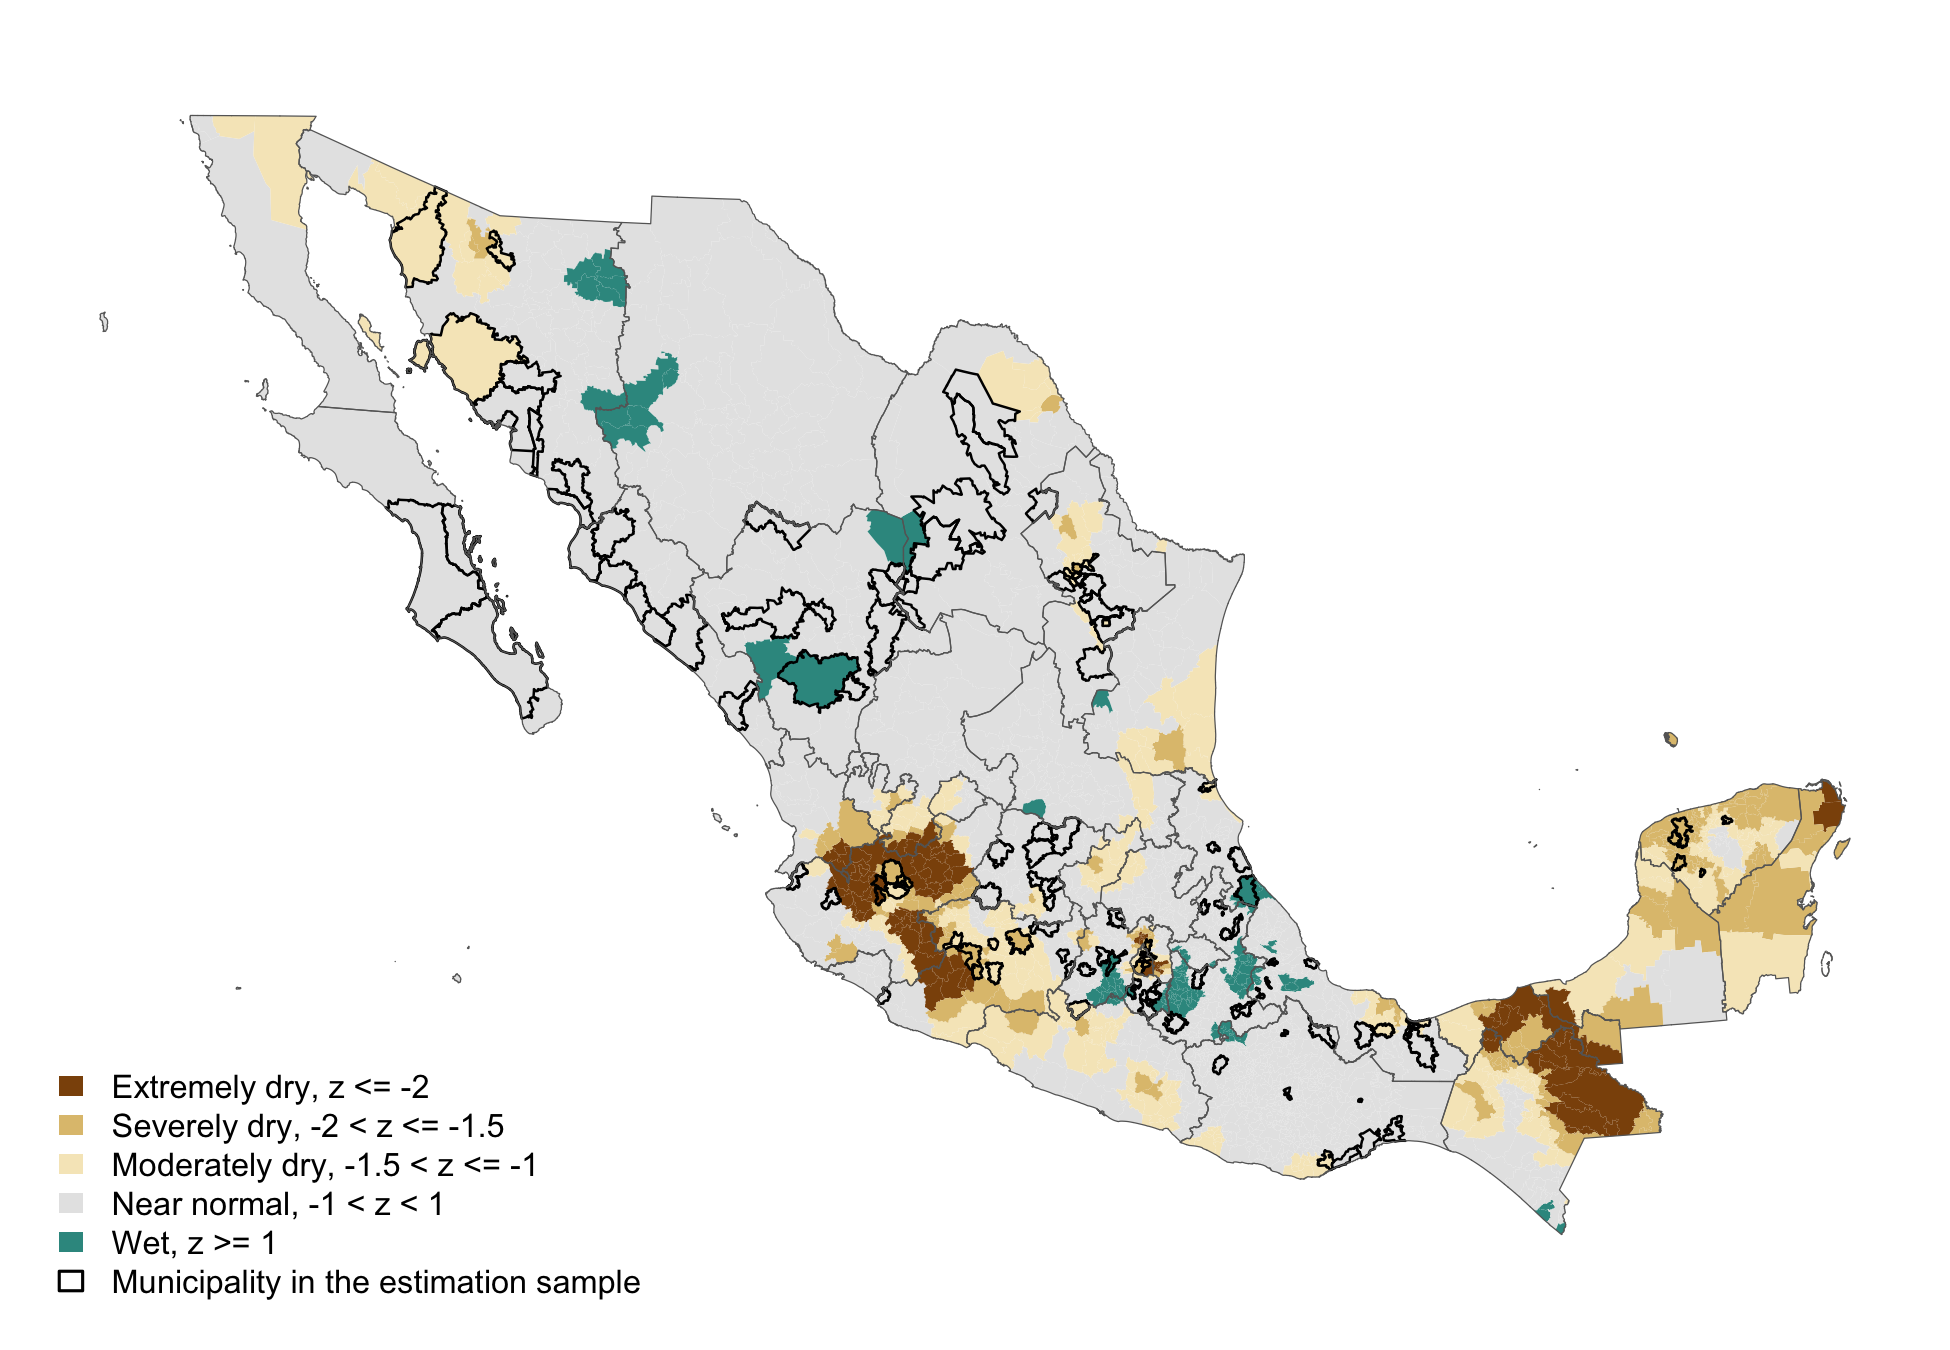
\includegraphics[width=0.8\textwidth]{drought_map_spi.png}
\end{figure}

\begin{figure}[H]
\centering
\caption{Event Study by Dose Level, BMI-for-Age, Discrete Dose}
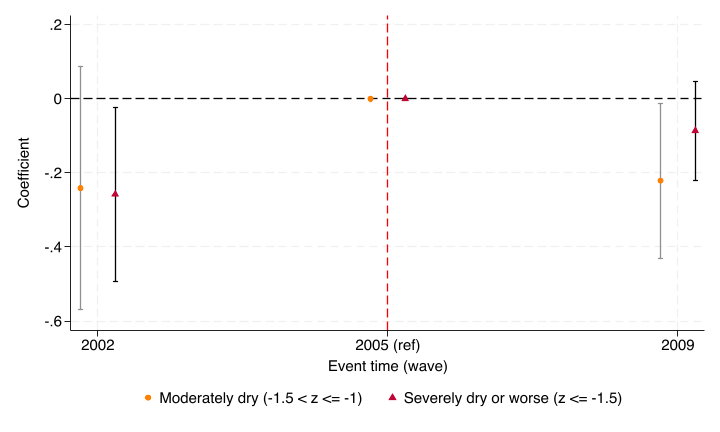
\includegraphics[width=0.8\textwidth]{event_study_severity_bmiz.png}
\par\parbox{0.8\textwidth}{\scriptsize \textit{Notes:} Moderately dry and severely dry or worse compared with near-normal. The 2009 coefficients are the same as in the discrete-dose table. Here I include both the 2002 lead and the 2009 coefficient. Similar to the discrete-dose table, there are no controls. Included are child and survey wave fixed effects. 2005 is the reference wave. 95\% confidence intervals use standard errors clustered by 2005 municipality.}
\end{figure}

\begin{figure}[H]
\centering
\caption{Event Study by Dose Level, Height-for-Age, Discrete Dose}
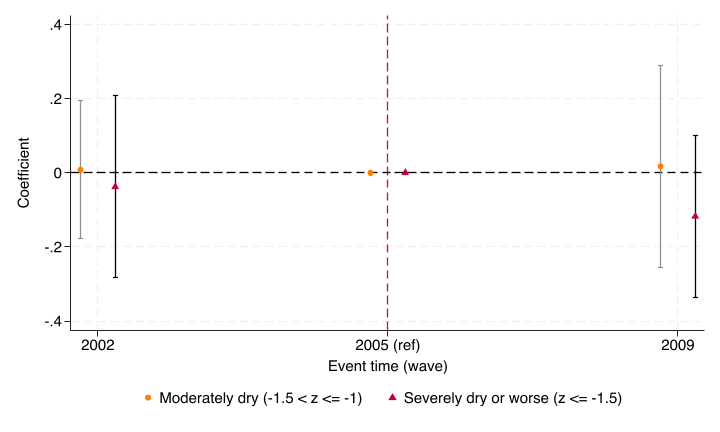
\includegraphics[width=0.8\textwidth]{event_study_severity_haz.png}
\par\parbox{0.8\textwidth}{\scriptsize \textit{Notes:} Moderately dry and severely dry or worse compared with near-normal. The 2009 coefficients are the same as in the discrete-dose table. Here I include both the 2002 lead and the 2009 coefficient. Similar to the discrete-dose table, there are no controls. Included are child and survey wave fixed effects. 2005 is the reference wave. 95\% confidence intervals use standard errors clustered by 2005 municipality.}
\end{figure}

\begin{figure}[H]
\centering
\caption{Event Study by Dose Level, Weight-for-Age, Discrete Dose}
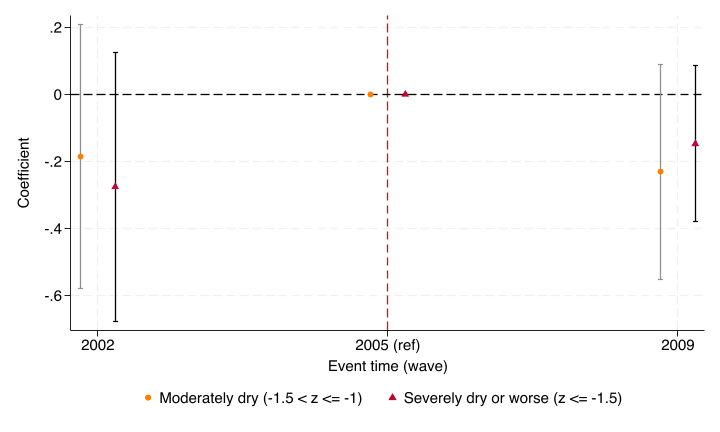
\includegraphics[width=0.8\textwidth]{event_study_severity_waz.png}
\par\parbox{0.8\textwidth}{\scriptsize \textit{Notes:} Moderately dry and severely dry or worse compared with near-normal. The 2009 coefficients are the same as in the discrete-dose table. Here I include both the 2002 lead and the 2009 coefficient. Similar to the discrete-dose table, there are no controls. Included are child and survey wave fixed effects. 2005 is the reference wave. 95\% confidence intervals use standard errors clustered by 2005 municipality.}
\end{figure}

\begin{figure}[H]
\centering
\caption{Event Study by Dose Level, BMI-for-Age, Discrete Dose, Children in All Three Waves}
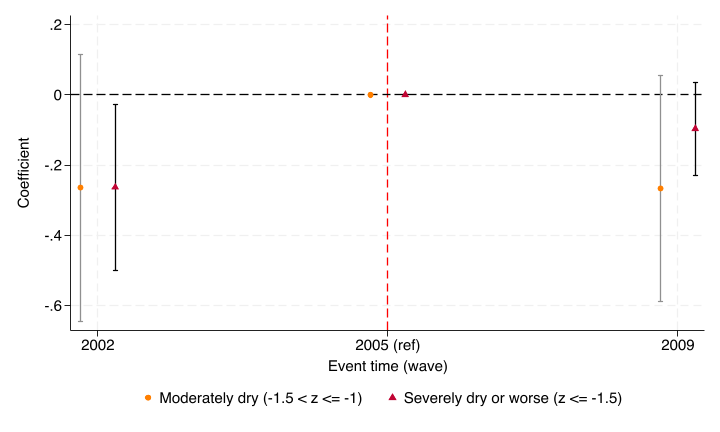
\includegraphics[width=0.8\textwidth]{event_study_severity_bmiz_all3.png}
\par\parbox{0.8\textwidth}{\scriptsize \textit{Notes:} Moderately dry and severely dry or worse compared with near-normal. The sample is the children in the discrete-dose table who were measured in all three survey waves, so the 2002 lead and the 2009 coefficient come from the same children. Similar to the discrete-dose table, there are no controls. Included are child and survey wave fixed effects. 2005 is the reference wave. 95\% confidence intervals use standard errors clustered by 2005 municipality.}
\end{figure}

\begin{figure}[H]
\centering
\caption{Overlap of Baseline Characteristics, BMI-for-Age, Dose Groups}
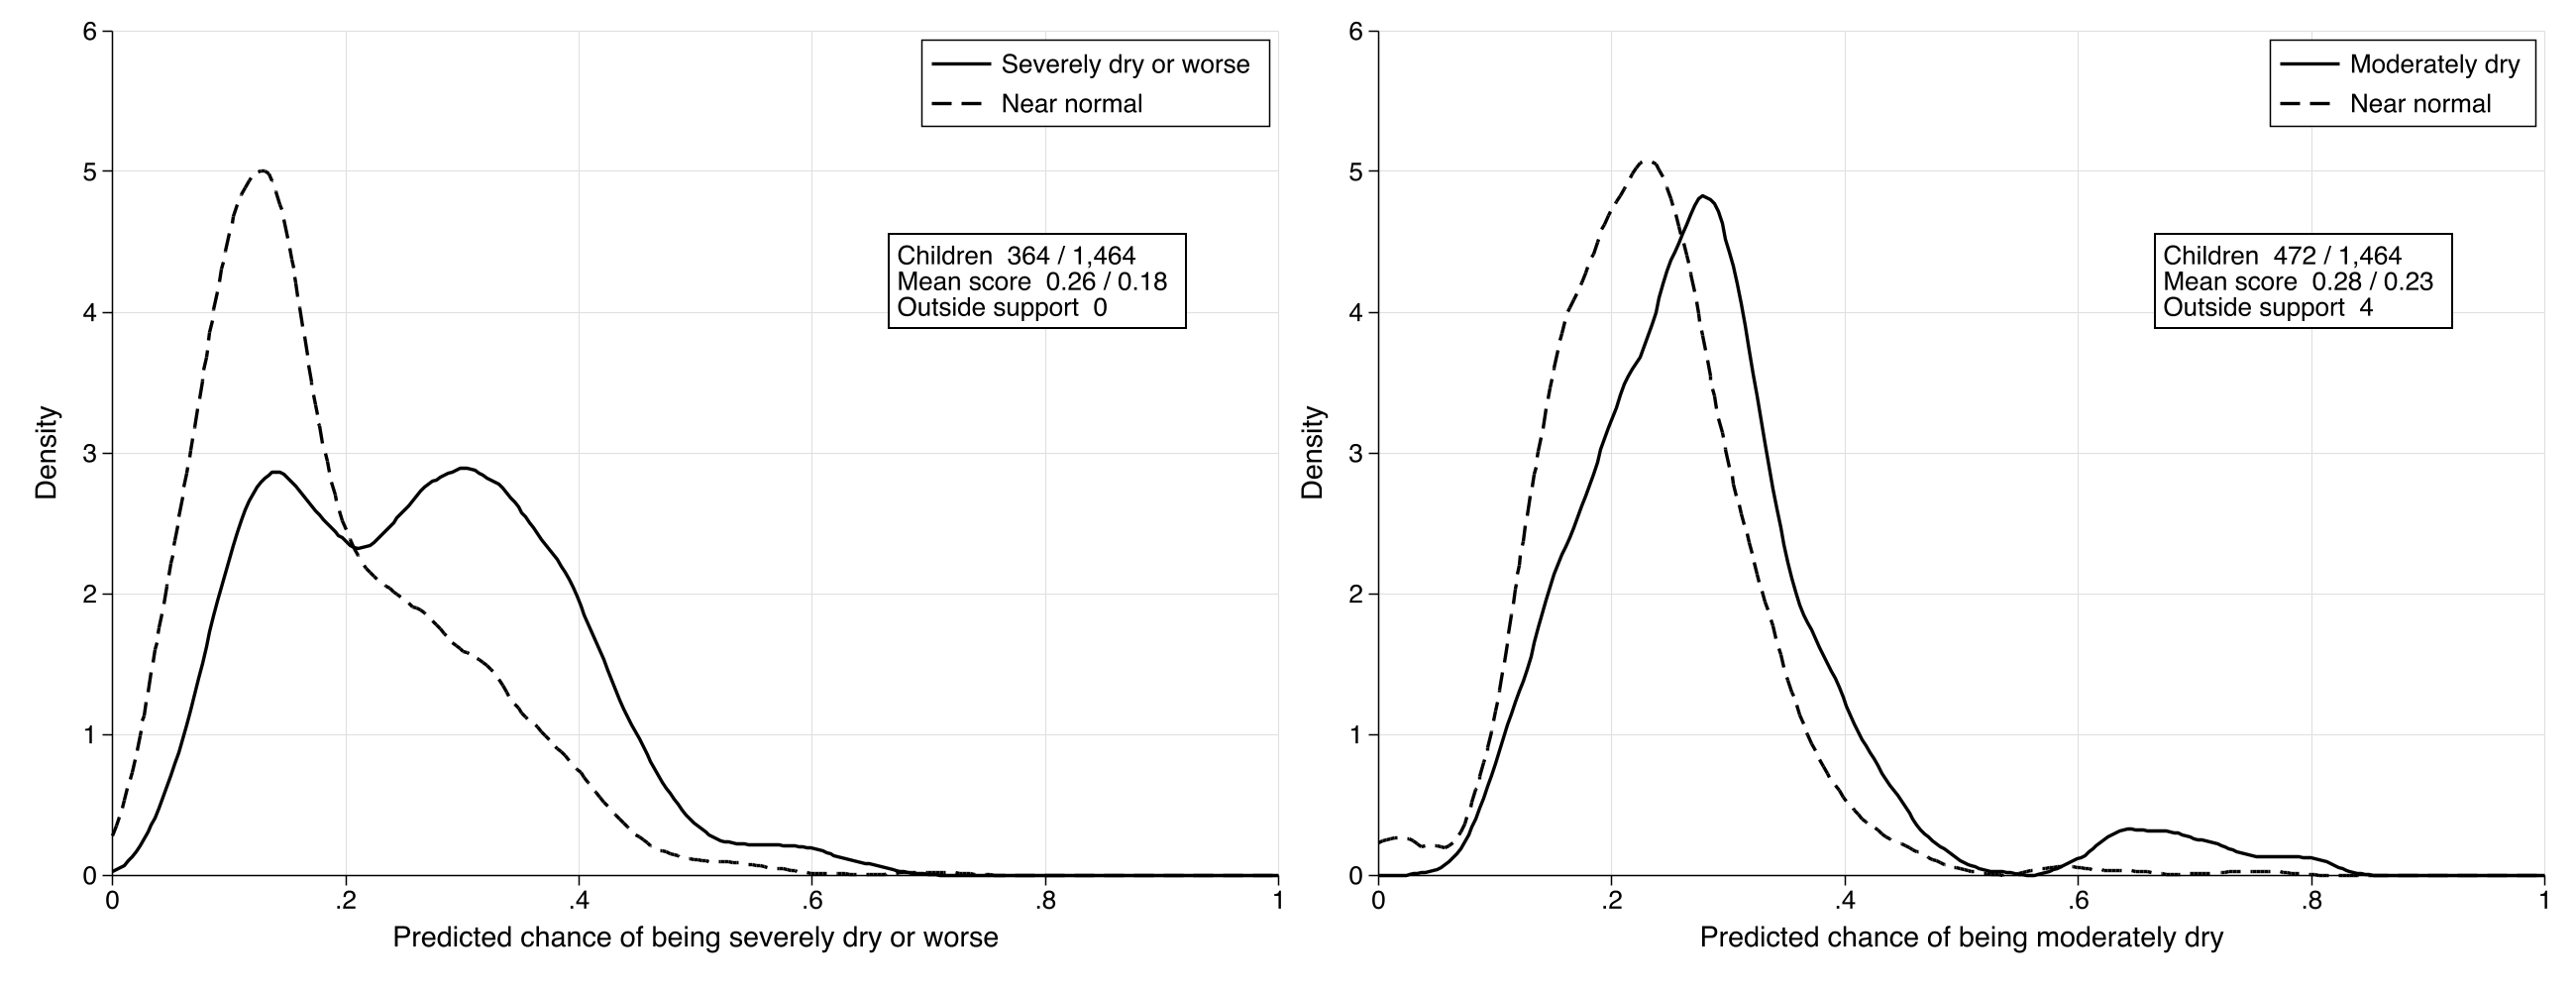
\includegraphics[width=0.8\textwidth]{overlap_pscore_bmiz.png}
\par\parbox{0.8\textwidth}{\scriptsize \textit{Notes:} The sample is the children in the discrete-dose regressions. Kernel densities of the propensity score. That is, the predicted probability of being in the dry dose group from a logit on baseline characteristics. Baseline characteristics are the 2002 household controls (electricity, floor, roof, ventilation, rooms per person, log expenditure per person, rural) and the 2005 child and mother controls (sex, full vaccination, mother's height, schooling, age at birth, and employment), and the child's age. Missing values are set to the sample mean and flagged with an indicator. Each panel compares one dry dose group with near-normal (\ensuremath{-1<z<1}) and is estimated separately. Moderately dry is \ensuremath{-1.5<z\le -1}, and severely dry or worse is \ensuremath{z\le -1.5}. In each box, children and mean score are shown as dry dose group/near-normal. Outside support is the number of dry dose group children whose score lies below the lowest or above the highest near-normal score.}
\end{figure}

\clearpage
\section*{Appendix}

\begingroup
\footnotesize
\renewcommand{\arraystretch}{0.86}
\setlength{\tabcolsep}{4pt}
\setlength{\LTcapwidth}{\textwidth}
\begin{longtable}{l*{6}{c}}
\caption{Summary Statistics, Binary DID Model 3 Samples}\\
\toprule
 & \multicolumn{6}{c}{Panel A: WAZ, age \ensuremath{\le}10 in 2005 and 2009}\\
\cmidrule(lr){2-7}
                    &        Mean&   Std. dev.&        Min.&      Median&        Max.&        Obs.\\
\midrule
\textit{Outcomes (MxFLS-2, 2005)}&            &            &            &            &            &            \\
Weight-for-age z-score (WAZ)&       -0.31&        1.40&       -4.92&       -0.34&        4.51&         700\\
\addlinespace[6pt]\textit{Binary DID treatment (CHIRPS)}&            &            &            &            &            &            \\
2009 drought (indicator)&        0.36&        0.48&        0.00&        0.00&        1.00&         700\\
2005 drought (indicator)&        0.68&        0.47&        0.00&        1.00&        1.00&         700\\
2006 drought (indicator)&        0.03&        0.17&        0.00&        0.00&        1.00&         700\\
2007 drought (indicator)&        0.15&        0.36&        0.00&        0.00&        1.00&         700\\
2008 drought (indicator)&        0.13&        0.34&        0.00&        0.00&        1.00&         700\\
\addlinespace[6pt]\textit{Remittances (MxFLS-1, 2002)}&            &            &            &            &            &            \\
Household received remittances, proxy (indicator)&        0.41&        0.49&        0.00&        0.00&        1.00&         634\\
\addlinespace[6pt]\textit{Household (MxFLS-1, 2002)}&            &            &            &            &            &            \\
Dwelling has electricity (indicator)&        0.97&        0.16&        0.00&        1.00&        1.00&         700\\
Good floor quality (indicator)&        0.85&        0.36&        0.00&        1.00&        1.00&         700\\
Good roof quality (indicator)&        0.81&        0.39&        0.00&        1.00&        1.00&         700\\
Enough ventilation (indicator)&        0.57&        0.50&        0.00&        1.00&        1.00&         700\\
Sleeping rooms per household member&        0.41&        0.25&        0.11&        0.33&        2.33&         700\\
Ln (monthly expenditure per capita, pesos), proxy&        6.56&        0.86&        4.21&        6.57&       11.43&         700\\
Rural locality (indicator)&        0.43&        0.50&        0.00&        0.00&        1.00&         700\\
\addlinespace[6pt]\textit{Child and mother (MxFLS-2, 2005)}&            &            &            &            &            &            \\
Age (years, not in regression)&        2.52&        1.68&        0.00&        3.00&        6.00&         700\\
Male (indicator)    &        0.53&        0.50&        0.00&        1.00&        1.00&         700\\
Fully vaccinated (indicator)&        0.39&        0.49&        0.00&        0.00&        1.00&         700\\
Mother's height (centimeters)&      154.79&        6.91&      136.00&      154.50&      181.00&         700\\
Mother's years of schooling&        7.40&        3.42&        0.00&        8.00&       18.00&         700\\
Mother's age at birth (years)&       26.93&        6.52&       14.00&       27.00&       59.00&         700\\
Mother employed (indicator)&        0.24&        0.42&        0.00&        0.00&        1.00&         700\\
\addlinespace[6pt]\textit{Father and birth (MxFLS-1 and MxFLS-2)}&            &            &            &            &            &            \\
Father's height (centimeters)&      166.81&        6.98&      144.00&      167.00&      189.40&         465\\
Father's years of schooling&        7.51&        3.77&        0.00&        8.00&       18.00&         569\\
Father's age at birth (years)&       30.74&        7.82&       16.00&       30.00&       75.00&         581\\
Father employed (indicator)&        0.96&        0.19&        0.00&        1.00&        1.00&         569\\
Birth order         &        2.31&        1.68&        1.00&        2.00&       13.00&         401\\
Oldest child (indicator)&        0.40&        0.49&        0.00&        0.00&        1.00&         401\\
Birth weight (kilograms)&        3.26&        0.59&        1.55&        3.20&        5.50&         523\\
Delivered at home (indicator)&        0.08&        0.27&        0.00&        0.00&        1.00&         560\\
Weeks predominantly breastfed&       31.98&       29.20&        0.00&       26.09&      157.29&         542\\
Iron during pregnancy (indicator)&        0.76&        0.43&        0.00&        1.00&        1.00&         549\\
Premature, mother reported (indicator)&        0.19&        0.39&        0.00&        0.00&        1.00&         546\\

\bottomrule
\newpage
\toprule
 & \multicolumn{6}{c}{Panel B: HAZ and BMIZ, age \ensuremath{\le}15 in 2005 and 2009}\\
\cmidrule(lr){2-7}
                    &        Mean&   Std. dev.&        Min.&      Median&        Max.&        Obs.\\
\midrule
\textit{Outcomes (MxFLS-2, 2005)}&            &            &            &            &            &            \\
Height-for-age z-score (HAZ)&       -0.60&        1.47&       -5.17&       -0.62&        5.20&       1,755\\
BMI-for-age z-score (BMIZ)&        0.40&        1.41&       -4.95&        0.35&        4.86&       1,721\\
\addlinespace[6pt]\textit{Binary DID treatment (CHIRPS)}&            &            &            &            &            &            \\
2009 drought (indicator)&        0.39&        0.49&        0.00&        0.00&        1.00&       1,755\\
2005 drought (indicator)&        0.66&        0.47&        0.00&        1.00&        1.00&       1,755\\
2006 drought (indicator)&        0.03&        0.17&        0.00&        0.00&        1.00&       1,755\\
2007 drought (indicator)&        0.16&        0.36&        0.00&        0.00&        1.00&       1,755\\
2008 drought (indicator)&        0.14&        0.34&        0.00&        0.00&        1.00&       1,755\\
\addlinespace[6pt]\textit{Remittances (MxFLS-1, 2002)}&            &            &            &            &            &            \\
Household received remittances, proxy (indicator)&        0.36&        0.48&        0.00&        0.00&        1.00&       1,624\\
\addlinespace[6pt]\textit{Household (MxFLS-1, 2002)}&            &            &            &            &            &            \\
Dwelling has electricity (indicator)&        0.98&        0.15&        0.00&        1.00&        1.00&       1,755\\
Good floor quality (indicator)&        0.83&        0.37&        0.00&        1.00&        1.00&       1,755\\
Good roof quality (indicator)&        0.81&        0.39&        0.00&        1.00&        1.00&       1,755\\
Enough ventilation (indicator)&        0.56&        0.50&        0.00&        1.00&        1.00&       1,755\\
Sleeping rooms per household member&        0.38&        0.23&        0.11&        0.33&        2.33&       1,755\\
Ln (monthly expenditure per capita, pesos), proxy&        6.52&        0.86&        3.75&        6.51&       12.24&       1,755\\
Rural locality (indicator)&        0.46&        0.50&        0.00&        0.00&        1.00&       1,755\\
\addlinespace[6pt]\textit{Child and mother (MxFLS-2, 2005)}&            &            &            &            &            &            \\
Age (years, not in regression)&        6.08&        3.22&        0.00&        6.00&       12.00&       1,755\\
Male (indicator)    &        0.50&        0.50&        0.00&        0.00&        1.00&       1,755\\
Fully vaccinated (indicator)&        0.50&        0.50&        0.00&        0.00&        1.00&       1,755\\
Mother's height (centimeters)&      154.39&        7.14&      133.40&      154.20&      190.00&       1,755\\
Mother's years of schooling&        7.13&        3.66&        0.00&        6.00&       18.00&       1,755\\
Mother's age at birth (years)&       26.80&        6.46&       14.00&       26.00&       59.00&       1,755\\
Mother employed (indicator)&        0.28&        0.45&        0.00&        0.00&        1.00&       1,755\\
\addlinespace[6pt]\textit{Father and birth (MxFLS-1 and MxFLS-2)}&            &            &            &            &            &            \\
Father's height (centimeters)&      166.42&        7.15&      144.00&      166.30&      192.00&       1,212\\
Father's years of schooling&        7.33&        3.92&        0.00&        7.00&       18.00&       1,443\\
Father's age at birth (years)&       30.36&        7.85&       15.00&       29.00&       75.00&       1,482\\
Father employed (indicator)&        0.96&        0.20&        0.00&        1.00&        1.00&       1,447\\
Birth order         &        2.66&        1.89&        1.00&        2.00&       13.00&       1,392\\
Oldest child (indicator)&        0.32&        0.47&        0.00&        0.00&        1.00&       1,392\\
Birth weight (kilograms)&        3.27&        0.60&        0.85&        3.25&        6.00&       1,256\\
Delivered at home (indicator)&        0.12&        0.32&        0.00&        0.00&        1.00&       1,544\\
Weeks predominantly breastfed&       33.57&       33.98&        0.00&       26.09&      260.89&       1,357\\
Iron during pregnancy (indicator)&        0.72&        0.45&        0.00&        1.00&        1.00&       1,366\\
Premature, mother reported (indicator)&        0.14&        0.35&        0.00&        0.00&        1.00&       1,362\\

\bottomrule
\addlinespace[6pt]\multicolumn{7}{p{0.97\textwidth}}{\scriptsize \textit{Notes:} This table is for the sample of Model 3, the main binary DID with controls. Obs. counts children. The children have the outcome measured in MxFLS-2 (2005) and MxFLS-3 (2009), under the panel's age cutoff
in both survey waves, and a 2005 municipality. They were not measured in MxFLS-3 before November 2009, for the same reason as in Table~\ref{tab:sumstats}.
Panel A uses the WAZ sample, Panel B the HAZ and BMIZ sample. The BMIZ sample is marginally smaller than the HAZ sample shown in Panel B, at 1,714 children. Statistics are at the 2005 baseline, except remittances and household variables (2002). Remittances enter Model 5, and the father and birth controls enter Model 4. Both are observed for fewer children.
Drought is May--October CHIRPS rainfall, the maize growing season (Jessoe, Manning, and Taylor 2018), in the 2005 municipality below its 1981--2004 20th percentile (Shah and Steinberg 2017). Remittances are cash received in the last
12 months from parents, siblings, or children outside the household. Expenditure is in 2002 pesos per person per month.
Rural is a locality under 2,500 inhabitants (INEGI 2024).}\\
\end{longtable}
\endgroup

\clearpage
\begingroup
\footnotesize
\renewcommand{\arraystretch}{0.86}
\setlength{\tabcolsep}{4pt}
\setlength{\LTcapwidth}{\textwidth}
\begin{longtable}{p{0.62\textwidth}ccc}
\caption{2009 Drought and Child Anthropometrics, Binary DID Model 3 with All Covariates}\\
\toprule
 & HAZ & WAZ & BMIZ\\
            &\multicolumn{1}{c}{(1)}         &\multicolumn{1}{c}{(2)}         &\multicolumn{1}{c}{(3)}         \\
\midrule
2009 drought \ensuremath{\times} post&       0.021         &      -0.299\sym{**} &      -0.304\sym{***}\\
            &     (0.113)         &     (0.125)         &     (0.095)         \\
2005 drought \ensuremath{\times} post&       0.127         &      -0.193         &      -0.129         \\
            &     (0.114)         &     (0.124)         &     (0.085)         \\
2006 drought \ensuremath{\times} post&      -0.254         &      -0.343         &      -0.043         \\
            &     (0.158)         &     (0.294)         &     (0.199)         \\
2007 drought \ensuremath{\times} post&      -0.137         &      -0.181         &      -0.202\sym{*}  \\
            &     (0.118)         &     (0.152)         &     (0.120)         \\
2008 drought \ensuremath{\times} post&      -0.070         &       0.037         &       0.350\sym{**} \\
            &     (0.154)         &     (0.181)         &     (0.138)         \\
2002 dwelling has electricity \ensuremath{\times} post&      -0.707\sym{**} &      -0.494\sym{**} &       0.016         \\
            &     (0.321)         &     (0.211)         &     (0.239)         \\
2002 good floor quality \ensuremath{\times} post&      -0.140         &      -0.031         &       0.137         \\
            &     (0.114)         &     (0.156)         &     (0.102)         \\
2002 good roof quality \ensuremath{\times} post&       0.083         &      -0.161         &      -0.155         \\
            &     (0.093)         &     (0.160)         &     (0.099)         \\
2002 enough ventilation \ensuremath{\times} post&       0.057         &      -0.010         &       0.140\sym{**} \\
            &     (0.077)         &     (0.124)         &     (0.065)         \\
2002 sleeping rooms per member \ensuremath{\times} post&       0.116         &       0.224         &       0.258\sym{*}  \\
            &     (0.187)         &     (0.255)         &     (0.146)         \\
2002 ln expenditure per capita \ensuremath{\times} post&       0.023         &       0.147\sym{**} &      -0.044         \\
            &     (0.053)         &     (0.064)         &     (0.042)         \\
2002 rural locality \ensuremath{\times} post&      -0.137         &      -0.033         &       0.016         \\
            &     (0.096)         &     (0.115)         &     (0.073)         \\
Male \ensuremath{\times} post&       0.089         &       0.021         &      -0.000         \\
            &     (0.069)         &     (0.103)         &     (0.061)         \\
2005 mother's height (cm) \ensuremath{\times} post&      -0.009         &      -0.005         &      -0.001         \\
            &     (0.006)         &     (0.008)         &     (0.005)         \\
2005 mother's years of schooling \ensuremath{\times} post&       0.008         &       0.023         &       0.015         \\
            &     (0.012)         &     (0.015)         &     (0.011)         \\
Mother's age at birth \ensuremath{\times} post&      -0.002         &       0.005         &      -0.001         \\
            &     (0.006)         &     (0.007)         &     (0.005)         \\
2005 mother employed \ensuremath{\times} post&      -0.033         &      -0.171         &      -0.011         \\
            &     (0.077)         &     (0.117)         &     (0.079)         \\
2005 fully vaccinated \ensuremath{\times} post&      -0.020         &       0.282\sym{***}&       0.053         \\
            &     (0.086)         &     (0.105)         &     (0.064)         \\
\midrule
Child FE    &           Y         &           Y         &           Y         \\
Interview year-month FE&           Y         &           Y         &           Y         \\
Children    &       1,755         &         700         &       1,714         \\
2005 municipalities (clusters)&         116         &         101         &         116         \\
\bottomrule
\addlinespace[6pt]\multicolumn{4}{p{0.97\textwidth}}{\scriptsize \textit{Notes:} This table reports every coefficient of Model 3, which is Col. 3 of the main binary DID tables, including all control variables. All regressions include child and interview year-month fixed effects, children in singleton cells are dropped, and standard errors are clustered by 2005 municipality. \mbox{\sym{*}\(p<.10\), \sym{**}\(p<.05\), \sym{***}\(p<.01\).}}\\
\end{longtable}
\endgroup
\clearpage
\begingroup
\footnotesize
\renewcommand{\arraystretch}{0.86}
\setlength{\tabcolsep}{4pt}
\setlength{\LTcapwidth}{\textwidth}
\begin{longtable}{l*{5}{c}}
\caption{2009 Drought and Height-for-Age, Binary DID, All Three Waves}\\
\toprule
 & \multicolumn{5}{c}{Height-for-age z-score (HAZ)}\\
\cmidrule(lr){2-6}
            &\multicolumn{1}{c}{(1)}         &\multicolumn{1}{c}{(2)}         &\multicolumn{1}{c}{(3)}         &\multicolumn{1}{c}{(4)}         &\multicolumn{1}{c}{(5)}         \\
\midrule
Drought \ensuremath{\times} post&       0.023         &       0.048         &       0.144         &       0.099         &       0.181\sym{*}  \\
            &     (0.087)         &     (0.090)         &     (0.090)         &     (0.136)         &     (0.103)         \\
Drought \ensuremath{\times} post \ensuremath{\times} 2002 remittances&                     &                     &                     &                     &      -0.166         \\
            &                     &                     &                     &                     &     (0.141)         \\
2002 remittances \ensuremath{\times} post&                     &                     &                     &                     &      -0.084         \\
            &                     &                     &                     &                     &     (0.092)         \\
\midrule
2005--2008 droughts \ensuremath{\times} post&           N         &           Y         &           Y         &           Y         &           Y         \\
2002 household controls \ensuremath{\times} post&           N         &           N         &           Y         &           Y         &           Y         \\
2005 child and mother controls \ensuremath{\times} post&           N         &           N         &           Y         &           Y         &           Y         \\
2005 father and birth controls \ensuremath{\times} post&           N         &           N         &           N         &           Y         &           N         \\
Child FE    &           Y         &           Y         &           Y         &           Y         &           Y         \\
Interview year-month FE&           Y         &           Y         &           Y         &           Y         &           Y         \\
Children    &       1,293         &       1,293         &       1,084         &         559         &       1,003         \\
\bottomrule
\addlinespace[6pt]\multicolumn{6}{p{0.97\textwidth}}{\scriptsize \textit{Notes:} This robustness check keeps only children measured in all three waves.
The table reports the effect of the 2009 drought on HAZ with the binary DID for these children. They are aged 15 or younger in both survey waves. They were not measured in MxFLS-3 before November 2009, for the same reason as in Table~\ref{tab:sumstats}. Columns, variables and controls are as in the main binary DID tables. All regressions include child and interview year-month fixed effects, and standard errors are clustered by 2005 municipality. \mbox{\sym{*}\(p<.10\), \sym{**}\(p<.05\), \sym{***}\(p<.01\).}}\\
\end{longtable}
\endgroup
\clearpage
\begingroup
\footnotesize
\renewcommand{\arraystretch}{0.86}
\setlength{\tabcolsep}{4pt}
\setlength{\LTcapwidth}{\textwidth}
\begin{longtable}{l*{5}{c}}
\caption{2009 Drought and Weight-for-Age, Binary DID, All Three Waves}\\
\toprule
 & \multicolumn{5}{c}{Weight-for-age z-score (WAZ)}\\
\cmidrule(lr){2-6}
            &\multicolumn{1}{c}{(1)}         &\multicolumn{1}{c}{(2)}         &\multicolumn{1}{c}{(3)}         &\multicolumn{1}{c}{(4)}         &\multicolumn{1}{c}{(5)}         \\
\midrule
Drought \ensuremath{\times} post&       0.025         &      -0.084         &       0.064         &       0.361         &       0.293         \\
            &     (0.136)         &     (0.176)         &     (0.183)         &     (0.266)         &     (0.233)         \\
Drought \ensuremath{\times} post \ensuremath{\times} 2002 remittances&                     &                     &                     &                     &      -0.444         \\
            &                     &                     &                     &                     &     (0.360)         \\
2002 remittances \ensuremath{\times} post&                     &                     &                     &                     &       0.149         \\
            &                     &                     &                     &                     &     (0.257)         \\
\midrule
2005--2008 droughts \ensuremath{\times} post&           N         &           Y         &           Y         &           Y         &           Y         \\
2002 household controls \ensuremath{\times} post&           N         &           N         &           Y         &           Y         &           Y         \\
2005 child and mother controls \ensuremath{\times} post&           N         &           N         &           Y         &           Y         &           Y         \\
2005 father and birth controls \ensuremath{\times} post&           N         &           N         &           N         &           Y         &           N         \\
Child FE    &           Y         &           Y         &           Y         &           Y         &           Y         \\
Interview year-month FE&           Y         &           Y         &           Y         &           Y         &           Y         \\
Children    &         266         &         266         &         203         &         121         &         179         \\
\bottomrule
\addlinespace[6pt]\multicolumn{6}{p{0.97\textwidth}}{\scriptsize \textit{Notes:} This robustness check keeps only children measured in all three waves.
The table reports the effect of the 2009 drought on WAZ with the binary DID for these children. They are aged 10 or younger in both survey waves. They were not measured in MxFLS-3 before November 2009, for the same reason as in Table~\ref{tab:sumstats}. Columns, variables and controls are as in the main binary DID tables. All regressions include child and interview year-month fixed effects, and standard errors are clustered by 2005 municipality. \mbox{\sym{*}\(p<.10\), \sym{**}\(p<.05\), \sym{***}\(p<.01\).}}\\
\end{longtable}
\endgroup
\clearpage
\begingroup
\footnotesize
\renewcommand{\arraystretch}{0.86}
\setlength{\tabcolsep}{4pt}
\setlength{\LTcapwidth}{\textwidth}
\begin{longtable}{l*{5}{c}}
\caption{2009 Drought and BMI-for-Age, Binary DID, All Three Waves}\\
\toprule
 & \multicolumn{5}{c}{BMI-for-age z-score (BMIZ)}\\
\cmidrule(lr){2-6}
            &\multicolumn{1}{c}{(1)}         &\multicolumn{1}{c}{(2)}         &\multicolumn{1}{c}{(3)}         &\multicolumn{1}{c}{(4)}         &\multicolumn{1}{c}{(5)}         \\
\midrule
Drought \ensuremath{\times} post&      -0.147         &      -0.223\sym{**} &      -0.250\sym{**} &      -0.171         &      -0.190         \\
            &     (0.089)         &     (0.107)         &     (0.118)         &     (0.121)         &     (0.147)         \\
Drought \ensuremath{\times} post \ensuremath{\times} 2002 remittances&                     &                     &                     &                     &      -0.032         \\
            &                     &                     &                     &                     &     (0.247)         \\
2002 remittances \ensuremath{\times} post&                     &                     &                     &                     &       0.012         \\
            &                     &                     &                     &                     &     (0.098)         \\
\midrule
2005--2008 droughts \ensuremath{\times} post&           N         &           Y         &           Y         &           Y         &           Y         \\
2002 household controls \ensuremath{\times} post&           N         &           N         &           Y         &           Y         &           Y         \\
2005 child and mother controls \ensuremath{\times} post&           N         &           N         &           Y         &           Y         &           Y         \\
2005 father and birth controls \ensuremath{\times} post&           N         &           N         &           N         &           Y         &           N         \\
Child FE    &           Y         &           Y         &           Y         &           Y         &           Y         \\
Interview year-month FE&           Y         &           Y         &           Y         &           Y         &           Y         \\
Children    &       1,196         &       1,196         &       1,006         &         513         &         933         \\
\bottomrule
\addlinespace[6pt]\multicolumn{6}{p{0.97\textwidth}}{\scriptsize \textit{Notes:} This robustness check keeps only children measured in all three waves.
The table reports the effect of the 2009 drought on BMIZ with the binary DID for these children. They are aged 15 or younger in both survey waves. They were not measured in MxFLS-3 before November 2009, for the same reason as in Table~\ref{tab:sumstats}. Columns, variables and controls are as in the main binary DID tables. All regressions include child and interview year-month fixed effects, and standard errors are clustered by 2005 municipality. \mbox{\sym{*}\(p<.10\), \sym{**}\(p<.05\), \sym{***}\(p<.01\).}}\\
\end{longtable}
\endgroup
\clearpage
\begingroup
\footnotesize
\renewcommand{\arraystretch}{0.86}
\setlength{\tabcolsep}{4pt}
\setlength{\LTcapwidth}{\textwidth}
\begin{longtable}{l*{2}{c}}
\caption{Event Study, 2009 Drought and Height-for-Age}\\
\toprule
 & \multicolumn{2}{c}{Height-for-age z-score (HAZ)}\\
\cmidrule(lr){2-3}
            &\multicolumn{1}{c}{(1)}&\multicolumn{1}{c}{(2)}\\
            &\multicolumn{1}{c}{Event study}&\multicolumn{1}{c}{Triple difference}\\
\midrule
Drought \ensuremath{\times} 2002 wave (lead)&       0.115         &       0.192         \\
            &     (0.116)         &     (0.128)         \\
Drought \ensuremath{\times} 2009 wave&       0.015         &      -0.008         \\
            &     (0.110)         &     (0.114)         \\
Drought \ensuremath{\times} 2002 remittances \ensuremath{\times} 2002 wave (lead)&                     &      -0.297         \\
            &                     &     (0.180)         \\
Drought \ensuremath{\times} 2002 remittances \ensuremath{\times} 2009 wave&                     &      -0.158         \\
            &                     &     (0.147)         \\
\midrule
2005--2008 droughts \ensuremath{\times} wave&           Y         &           Y         \\
2002 household controls \ensuremath{\times} wave&           Y         &           Y         \\
2005 child and mother controls \ensuremath{\times} wave&           Y         &           Y         \\
Child FE    &           Y         &           Y         \\
Interview year-month FE&           Y         &           Y         \\
P-value, lead = 0&       0.322         &       0.101         \\
\midrule 2009 drought effect, remittance households&                     &      -0.167         \\
\quad SE    &                     &       0.143         \\
\quad P-value&                     &       0.245         \\
\midrule Observations (child-waves)&       4,598         &       4,249         \\
Children    &       1,755         &       1,622         \\
2005 municipalities (clusters)&         116         &         114         \\
\bottomrule
\addlinespace[6pt]\multicolumn{3}{p{0.97\textwidth}}{\scriptsize \textit{Notes:} This table tests for pre-trends before the 2009 drought. Regressions are at the child-wave level with 2005 as the
reference wave. The sample is children aged 15 or younger in each wave they are in. They were not measured in MxFLS-3 before November 2009, for the same reason as in Table~\ref{tab:sumstats}. Col. 1 keeps the children in Model 3 of the binary DID and Col. 2 those in Model 5, so each matches its DID sample. Col. 1 interacts the drought indicator with the 2002 and 2009 waves. The 2002 interaction is the lead.
The 2005--2008 droughts and the 2002 household and 2005 child and mother controls are each interacted with both waves. Col. 2 adds the drought terms times 2002 remittances. The 2002 remittance terms on their own are not shown. The lead p-value tests the drought lead in Col. 1 and the triple difference lead in Col. 2.
Baseline controls are interacted with time to allow different trends by pre-treatment characteristics. The effect for remittance households is the sum of the two 2009 drought terms. All regressions include child and interview year-month fixed effects, and standard errors are clustered by 2005 municipality. \mbox{\sym{*}\(p<.10\), \sym{**}\(p<.05\), \sym{***}\(p<.01\).}}\\
\end{longtable}
\endgroup
\clearpage
\begingroup
\footnotesize
\renewcommand{\arraystretch}{0.86}
\setlength{\tabcolsep}{4pt}
\setlength{\LTcapwidth}{\textwidth}
\begin{longtable}{l*{2}{c}}
\caption{Event Study, 2009 Drought and Weight-for-Age}\\
\toprule
 & \multicolumn{2}{c}{Weight-for-age z-score (WAZ)}\\
\cmidrule(lr){2-3}
            &\multicolumn{1}{c}{(1)}&\multicolumn{1}{c}{(2)}\\
            &\multicolumn{1}{c}{Event study}&\multicolumn{1}{c}{Triple difference}\\
\midrule
Drought \ensuremath{\times} 2002 wave (lead)&      -0.481\sym{**} &      -0.336         \\
            &     (0.216)         &     (0.244)         \\
Drought \ensuremath{\times} 2009 wave&      -0.298\sym{**} &      -0.105         \\
            &     (0.126)         &     (0.145)         \\
Drought \ensuremath{\times} 2002 remittances \ensuremath{\times} 2002 wave (lead)&                     &      -0.078         \\
            &                     &     (0.347)         \\
Drought \ensuremath{\times} 2002 remittances \ensuremath{\times} 2009 wave&                     &      -0.373\sym{*}  \\
            &                     &     (0.208)         \\
\midrule
2005--2008 droughts \ensuremath{\times} wave&           Y         &           Y         \\
2002 household controls \ensuremath{\times} wave&           Y         &           Y         \\
2005 child and mother controls \ensuremath{\times} wave&           Y         &           Y         \\
Child FE    &           Y         &           Y         \\
Interview year-month FE&           Y         &           Y         \\
P-value, lead = 0&       0.028         &       0.822         \\
\midrule 2009 drought effect, remittance households&                     &      -0.477         \\
\quad SE    &                     &       0.200         \\
\quad P-value&                     &       0.019         \\
\midrule Observations (child-waves)&       1,609         &       1,454         \\
Children    &         700         &         634         \\
2005 municipalities (clusters)&         101         &          99         \\
\bottomrule
\addlinespace[6pt]\multicolumn{3}{p{0.97\textwidth}}{\scriptsize \textit{Notes:} This table tests for pre-trends before the 2009 drought. Regressions are at the child-wave level with 2005 as the
reference wave. The sample is children aged 10 or younger in each wave they are in. They were not measured in MxFLS-3 before November 2009, for the same reason as in Table~\ref{tab:sumstats}. Col. 1 keeps the children in Model 3 of the binary DID and Col. 2 those in Model 5, so each matches its DID sample. Col. 1 interacts the drought indicator with the 2002 and 2009 waves. The 2002 interaction is the lead.
The 2005--2008 droughts and the 2002 household and 2005 child and mother controls are each interacted with both waves. Col. 2 adds the drought terms times 2002 remittances. The 2002 remittance terms on their own are not shown. The lead p-value tests the drought lead in Col. 1 and the triple difference lead in Col. 2.
Baseline controls are interacted with time to allow different trends by pre-treatment characteristics. The effect for remittance households is the sum of the two 2009 drought terms. All regressions include child and interview year-month fixed effects, and standard errors are clustered by 2005 municipality. \mbox{\sym{*}\(p<.10\), \sym{**}\(p<.05\), \sym{***}\(p<.01\).}}\\
\end{longtable}
\endgroup
\clearpage
\begingroup
\footnotesize
\renewcommand{\arraystretch}{0.86}
\setlength{\tabcolsep}{4pt}
\setlength{\LTcapwidth}{\textwidth}
\begin{longtable}{l*{2}{c}}
\caption{Event Study, 2009 Drought and BMI-for-Age}\\
\toprule
 & \multicolumn{2}{c}{BMI-for-age z-score (BMIZ)}\\
\cmidrule(lr){2-3}
            &\multicolumn{1}{c}{(1)}&\multicolumn{1}{c}{(2)}\\
            &\multicolumn{1}{c}{Event study}&\multicolumn{1}{c}{Triple difference}\\
\midrule
Drought \ensuremath{\times} 2002 wave (lead)&      -0.387\sym{***}&      -0.423\sym{***}\\
            &     (0.104)         &     (0.120)         \\
Drought \ensuremath{\times} 2009 wave&      -0.293\sym{***}&      -0.262\sym{**} \\
            &     (0.097)         &     (0.114)         \\
Drought \ensuremath{\times} 2002 remittances \ensuremath{\times} 2002 wave (lead)&                     &       0.186         \\
            &                     &     (0.202)         \\
Drought \ensuremath{\times} 2002 remittances \ensuremath{\times} 2009 wave&                     &       0.040         \\
            &                     &     (0.217)         \\
\midrule
2005--2008 droughts \ensuremath{\times} wave&           Y         &           Y         \\
2002 household controls \ensuremath{\times} wave&           Y         &           Y         \\
2005 child and mother controls \ensuremath{\times} wave&           Y         &           Y         \\
Child FE    &           Y         &           Y         \\
Interview year-month FE&           Y         &           Y         \\
P-value, lead = 0&       0.000         &       0.358         \\
\midrule 2009 drought effect, remittance households&                     &      -0.222         \\
\quad SE    &                     &       0.167         \\
\quad P-value&                     &       0.187         \\
\midrule Observations (child-waves)&       4,438         &       4,110         \\
Children    &       1,714         &       1,587         \\
2005 municipalities (clusters)&         116         &         114         \\
\bottomrule
\addlinespace[6pt]\multicolumn{3}{p{0.97\textwidth}}{\scriptsize \textit{Notes:} This table tests for pre-trends before the 2009 drought. Regressions are at the child-wave level with 2005 as the
reference wave. The sample is children aged 15 or younger in each wave they are in. They were not measured in MxFLS-3 before November 2009, for the same reason as in Table~\ref{tab:sumstats}. Col. 1 keeps the children in Model 3 of the binary DID and Col. 2 those in Model 5, so each matches its DID sample. Col. 1 interacts the drought indicator with the 2002 and 2009 waves. The 2002 interaction is the lead.
The 2005--2008 droughts and the 2002 household and 2005 child and mother controls are each interacted with both waves. Col. 2 adds the drought terms times 2002 remittances. The 2002 remittance terms on their own are not shown. The lead p-value tests the drought lead in Col. 1 and the triple difference lead in Col. 2.
Baseline controls are interacted with time to allow different trends by pre-treatment characteristics. The effect for remittance households is the sum of the two 2009 drought terms. All regressions include child and interview year-month fixed effects, and standard errors are clustered by 2005 municipality. \mbox{\sym{*}\(p<.10\), \sym{**}\(p<.05\), \sym{***}\(p<.01\).}}\\
\end{longtable}
\endgroup

\clearpage
\begin{figure}[H]
\centering
\caption{2009 Drought by Municipality, Binary DID Treatment}
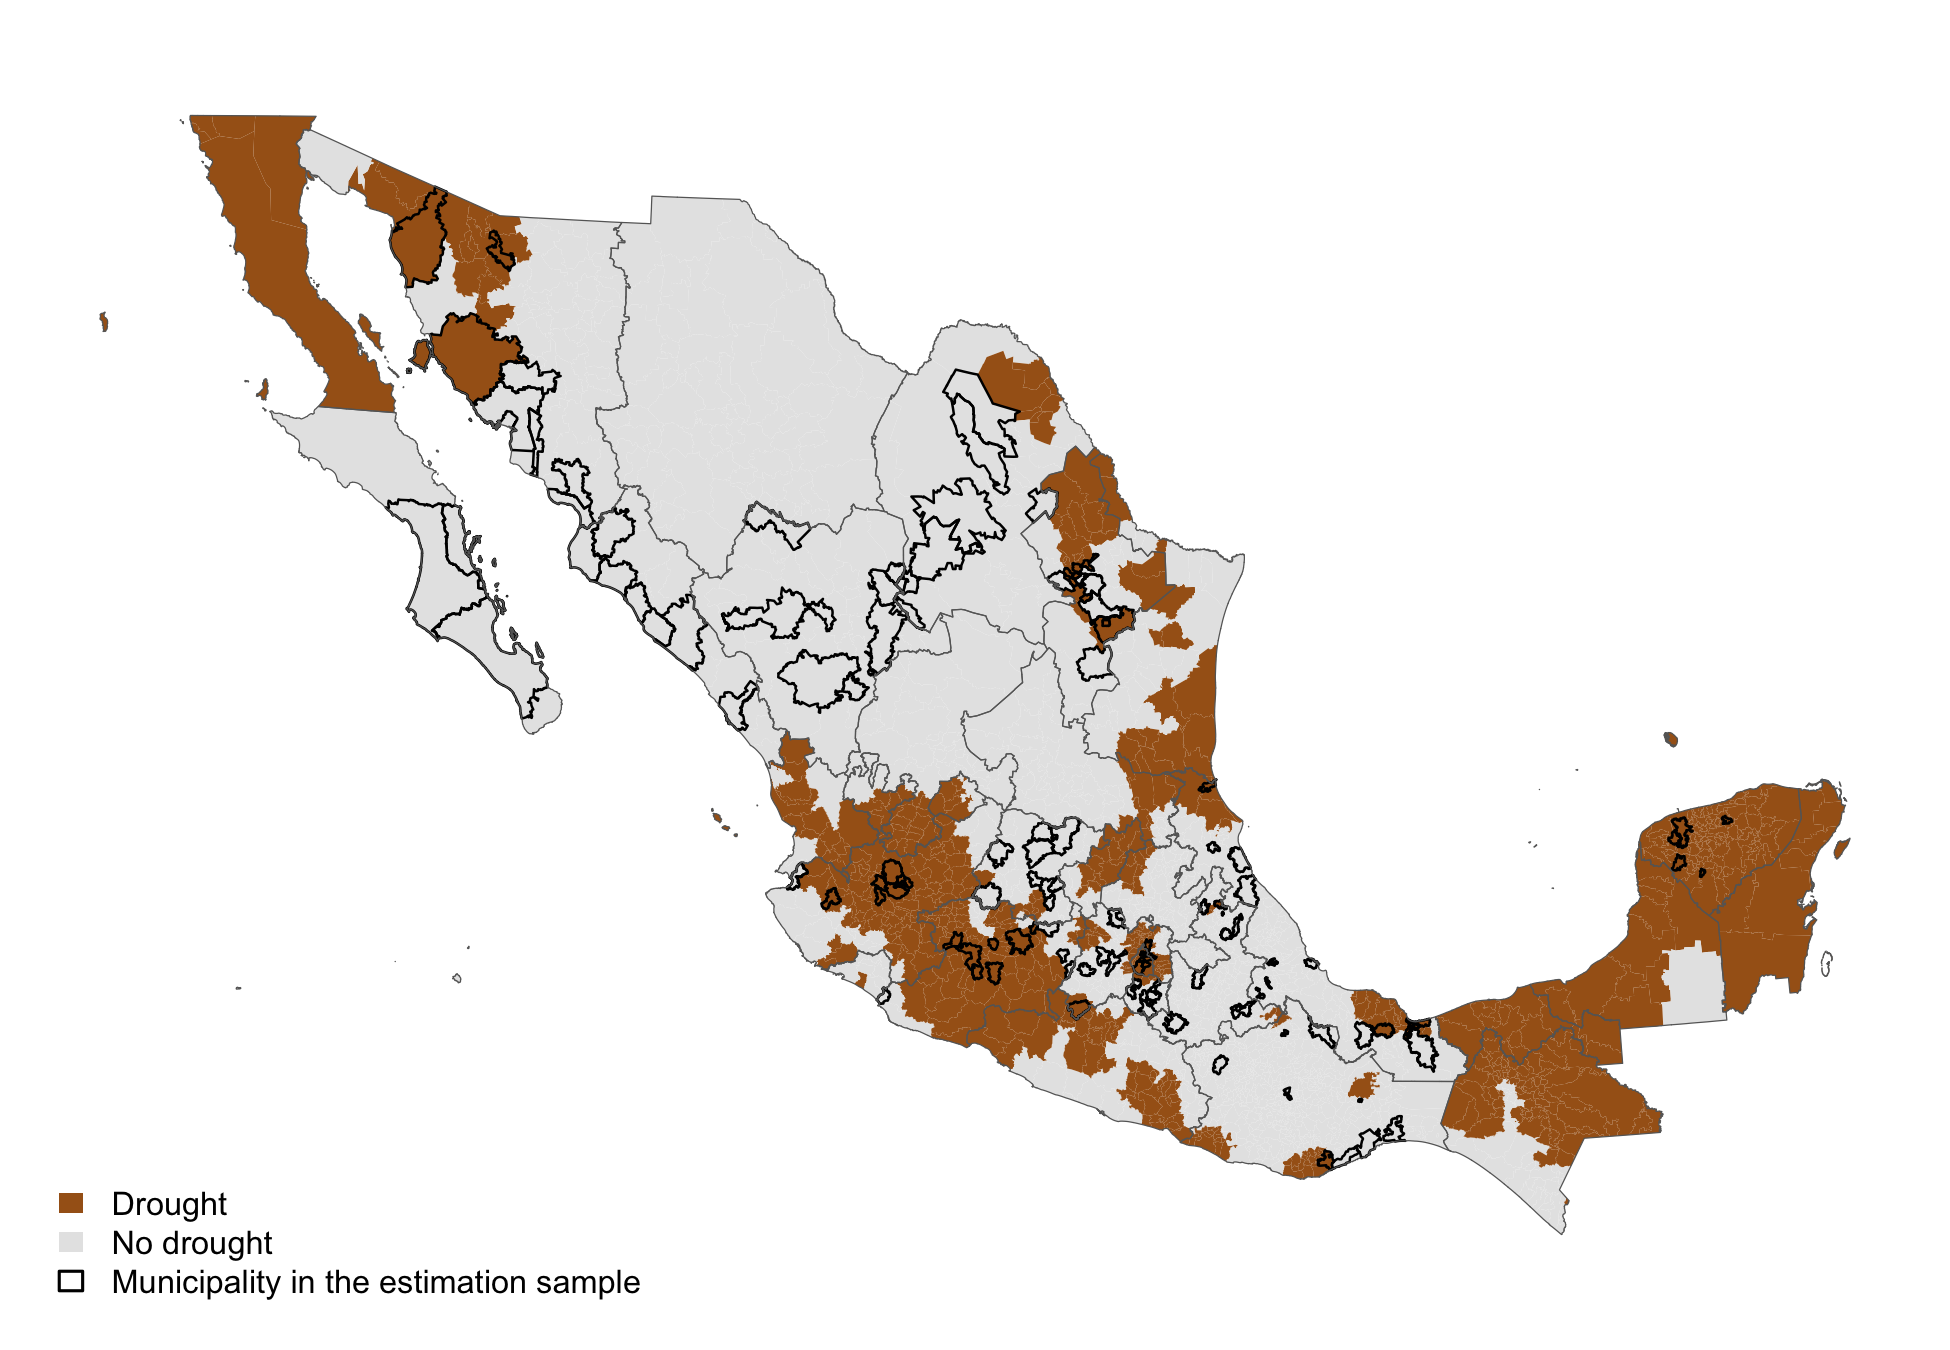
\includegraphics[width=0.8\textwidth]{drought_map_binary.png}
\end{figure}

\begin{figure}[H]
\centering
\caption{Event Study, BMI-for-Age, Binary DID, With Controls}
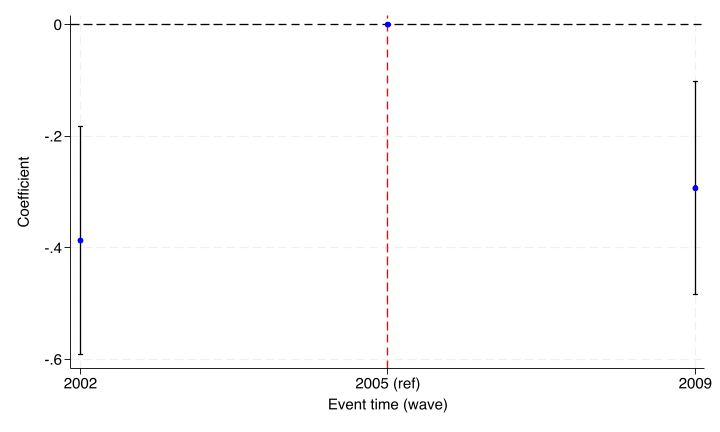
\includegraphics[width=0.8\textwidth]{event_study_bmiz_controls.png}
\par\parbox{0.8\textwidth}{\scriptsize \textit{Notes:} Drought compared with no drought. The coefficients are on the 2009 drought indicator interacted with the 2002 and 2009 survey waves. The sample is the children in Model 3 of the binary difference-in-differences, in each survey wave in which they are measured. The Model 3 controls are each interacted with the 2002 and 2009 survey waves. Included are child and interview year-month fixed effects. 2005 is the reference wave. 95\% confidence intervals use standard errors clustered by 2005 municipality.}
\end{figure}

\begin{figure}[H]
\centering
\caption{Event Study, Height-for-Age, Binary DID, With Controls}
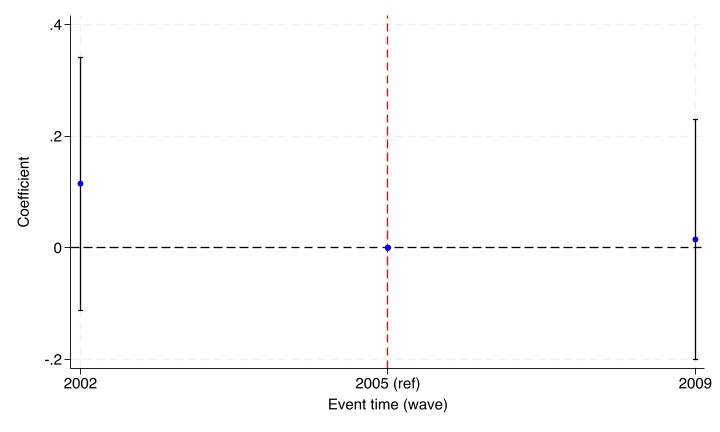
\includegraphics[width=0.8\textwidth]{event_study_haz_controls.png}
\par\parbox{0.8\textwidth}{\scriptsize \textit{Notes:} Drought compared with no drought. The coefficients are on the 2009 drought indicator interacted with the 2002 and 2009 survey waves. The sample is the children in Model 3 of the binary difference-in-differences, in each survey wave in which they are measured. The Model 3 controls are each interacted with the 2002 and 2009 survey waves. Included are child and interview year-month fixed effects. 2005 is the reference wave. 95\% confidence intervals use standard errors clustered by 2005 municipality.}
\end{figure}

\begin{figure}[H]
\centering
\caption{Event Study, Weight-for-Age, Binary DID, With Controls}
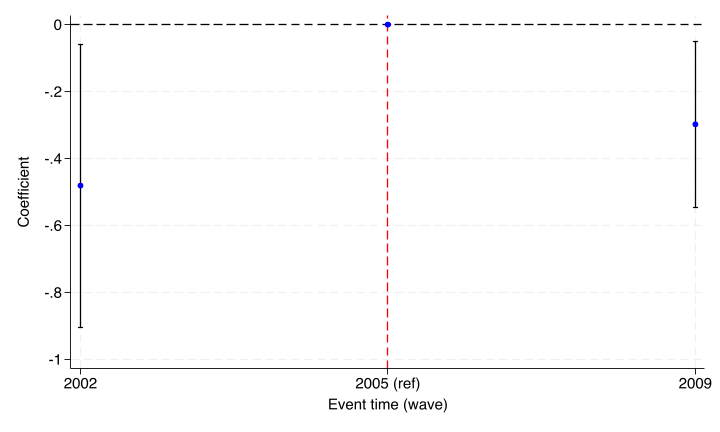
\includegraphics[width=0.8\textwidth]{event_study_waz_controls.png}
\par\parbox{0.8\textwidth}{\scriptsize \textit{Notes:} Drought compared with no drought. The coefficients are on the 2009 drought indicator interacted with the 2002 and 2009 survey waves. The sample is the children in Model 3 of the binary difference-in-differences, in each survey wave in which they are measured. The Model 3 controls are each interacted with the 2002 and 2009 survey waves. Included are child and interview year-month fixed effects. 2005 is the reference wave. 95\% confidence intervals use standard errors clustered by 2005 municipality.}
\end{figure}

\begin{figure}[H]
\centering
\caption{Event Study by Dose Level, Height-for-Age, Discrete Dose, Children in All Three Waves}
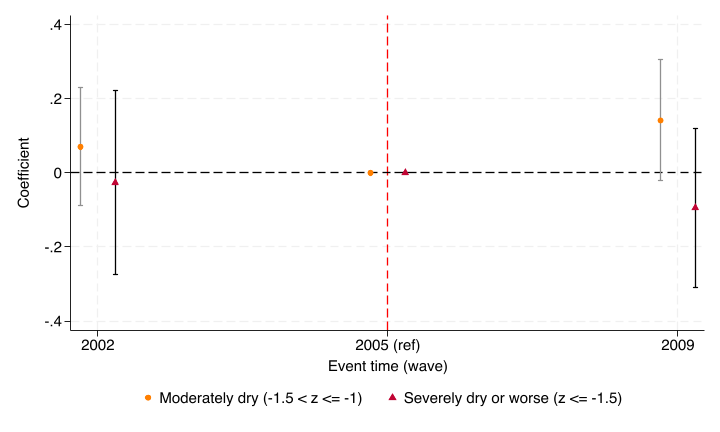
\includegraphics[width=0.8\textwidth]{event_study_severity_haz_all3.png}
\par\parbox{0.8\textwidth}{\scriptsize \textit{Notes:} Moderately dry and severely dry or worse compared with near-normal. The sample is the children in the discrete-dose table who were measured in all three survey waves, so the 2002 lead and the 2009 coefficient come from the same children. Similar to the discrete-dose table, there are no controls. Included are child and survey wave fixed effects. 2005 is the reference wave. 95\% confidence intervals use standard errors clustered by 2005 municipality.}
\end{figure}

\begin{figure}[H]
\centering
\caption{Event Study by Dose Level, Weight-for-Age, Discrete Dose, Children in All Three Waves}
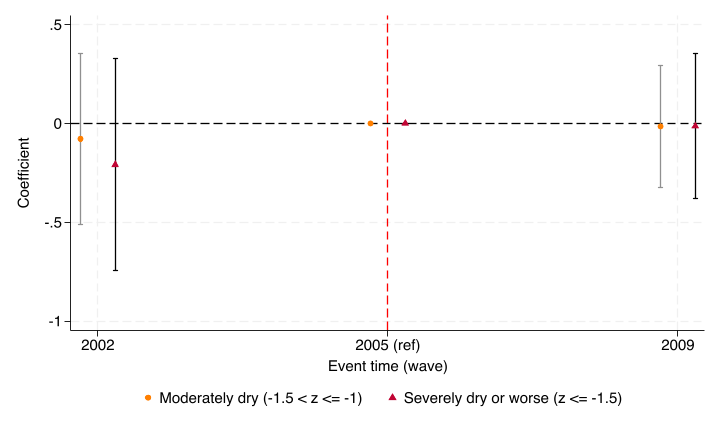
\includegraphics[width=0.8\textwidth]{event_study_severity_waz_all3.png}
\par\parbox{0.8\textwidth}{\scriptsize \textit{Notes:} Moderately dry and severely dry or worse compared with near-normal. The sample is the children in the discrete-dose table who were measured in all three survey waves, so the 2002 lead and the 2009 coefficient come from the same children. Similar to the discrete-dose table, there are no controls. Included are child and survey wave fixed effects. 2005 is the reference wave. 95\% confidence intervals use standard errors clustered by 2005 municipality.}
\end{figure}

\clearpage
\section*{Online Appendix}

\begingroup
\footnotesize
\renewcommand{\arraystretch}{0.86}
\setlength{\tabcolsep}{4pt}
\setlength{\LTcapwidth}{\textwidth}
\setlength{\LTleft}{0pt}
\setlength{\LTright}{0pt plus 1fil}
\begin{longtable}{@{\extracolsep{\fill}}lcc}
\caption{Sample Sizes, Treated and Control Children}\\
\toprule
 & \multicolumn{2}{c}{Panel A: Binary DID, 2009 drought}\\*
\cmidrule(lr){2-3}
 & Control & Treated\\*
\midrule
\textit{HAZ sample, children aged 15 or younger in 2005 and 2009} & & \\*
Children, estimation sample & 1,514 & 922\\*
Children, Model 1 (basic DID) & 1,512 & 920\\*
Children, Model 3 (DID with controls) & 1,077 & 678\\*
Children, Model 5 (triple difference) & 987 & 635\\*
\quad In 2002 remittance households & 390 & 193\\*
Households, estimation sample & 944 & 578\\*
2005 municipalities, estimation sample & 87 & 46\\
\addlinespace[6pt]\textit{WAZ sample, children aged 10 or younger in 2005 and 2009} & & \\*
Children, estimation sample & 696 & 388\\*
Children, Model 1 (basic DID) & 692 & 386\\*
Children, Model 3 (DID with controls) & 445 & 255\\*
Children, Model 5 (triple difference) & 400 & 234\\*
\quad In 2002 remittance households & 168 & 90\\*
Households, estimation sample & 565 & 316\\*
2005 municipalities, estimation sample & 79 & 44\\
\addlinespace[6pt]\textit{BMIZ sample, children aged 15 or younger in 2005 and 2009} & & \\*
Children, estimation sample & 1,487 & 896\\*
Children, Model 1 (basic DID) & 1,485 & 894\\*
Children, Model 3 (DID with controls) & 1,057 & 657\\*
Children, Model 5 (triple difference) & 968 & 619\\*
\quad In 2002 remittance households & 381 & 189\\*
Households, estimation sample & 931 & 561\\*
2005 municipalities, estimation sample & 87 & 46\\
\bottomrule
\addlinespace[12pt]
\toprule
 & \multicolumn{2}{c}{Panel B: Continuous DID, any 2009 deficit}\\*
\cmidrule(lr){2-3}
 & Control & Treated\\*
\midrule
\textit{HAZ sample, children aged 15 or younger in 2005 and 2009} & & \\*
Children, continuous DID sample & 829 & 1,607\\*
\quad In 2002 remittance households & 236 & 438\\*
\quad In 2002 non-remittance households & 437 & 738\\*
Households & 501 & 1,021\\*
2005 municipalities & 46 & 87\\
\addlinespace[6pt]\textit{WAZ sample, children aged 10 or younger in 2005 and 2009} & & \\*
Children, continuous DID sample & 380 & 704\\*
\quad In 2002 remittance households & 100 & 193\\*
\quad In 2002 non-remittance households & 172 & 260\\*
Households & 304 & 577\\*
2005 municipalities & 42 & 81\\
\addlinespace[6pt]\textit{BMIZ sample, children aged 15 or younger in 2005 and 2009} & & \\*
Children, continuous DID sample & 815 & 1,568\\*
\quad In 2002 remittance households & 231 & 427\\*
\quad In 2002 non-remittance households & 430 & 720\\*
Households & 496 & 996\\*
2005 municipalities & 46 & 87\\
\bottomrule
\newpage
\toprule
 & \multicolumn{2}{c}{Panel C: Dose groups vs near normal}\\*
\cmidrule(lr){2-3}
 & Control & Treated\\*
\midrule
\textit{Moderately dry, \ensuremath{-1.5<z\le -1}} & & \\*
Children, HAZ sample & 1,493 & 488\\*
Children, WAZ sample & 683 & 217\\*
Children, BMIZ sample & 1,464 & 472\\*
2005 municipalities, HAZ sample & 89 & 23\\*
2005 municipalities, WAZ sample & 80 & 23\\*
2005 municipalities, BMIZ sample & 89 & 23\\
\addlinespace[6pt]\textit{Severely dry or worse, \ensuremath{z\le -1.5}} & & \\*
Children, HAZ sample & 1,493 & 370\\*
Children, WAZ sample & 683 & 145\\*
Children, BMIZ sample & 1,464 & 364\\*
2005 municipalities, HAZ sample & 89 & 17\\*
2005 municipalities, WAZ sample & 80 & 16\\*
2005 municipalities, BMIZ sample & 89 & 17\\
\addlinespace[6pt]\textit{Severely dry, \ensuremath{-2<z\le -1.5}} & & \\*
Children, HAZ sample & 1,493 & 302\\*
Children, WAZ sample & 683 & 121\\*
Children, BMIZ sample & 1,464 & 296\\*
2005 municipalities, HAZ sample & 89 & 15\\*
2005 municipalities, WAZ sample & 80 & 14\\*
2005 municipalities, BMIZ sample & 89 & 15\\
\addlinespace[6pt]\textit{Extremely dry, \ensuremath{z\le -2}} & & \\*
Children, HAZ sample & 1,493 & 68\\*
Children, WAZ sample & 683 & 24\\*
Children, BMIZ sample & 1,464 & 68\\*
2005 municipalities, HAZ sample & 89 & 2\\*
2005 municipalities, WAZ sample & 80 & 2\\*
2005 municipalities, BMIZ sample & 89 & 2\\
\bottomrule
\addlinespace[6pt]\multicolumn{3}{p{0.97\textwidth}}{\scriptsize \textit{Notes:} Counts are children, households or 2005 municipalities in each regression sample at the 2005 baseline.
Estimation samples are children with the outcome measured in both MxFLS-2 (2005) and MxFLS-3 (2009) who have a 2005 municipality. They are aged 15 or younger for HAZ and BMIZ and 10 or younger for WAZ in both survey waves.
They were not measured in MxFLS-3 before November 2009, for the same reason as in Table~\ref{tab:sumstats}. In Panel A, treated children's 2005 municipality had a drought in 2009, meaning May--October CHIRPS rainfall in the maize growing season was below its 1981--2004 20th percentile
(Jessoe, Manning, and Taylor 2018; Shah and Steinberg 2017). Model 1 drops children alone in their interview-month cell. Continuous DID uses the full sample. Model 3 adds 2005--2008 droughts and 2002 household and 2005 child and mother controls.
Model 5 adds 2002 remittances times post and drought times post times 2002 remittances. Model 5 children not in remittance households are the Model 5 count minus the remittance row. In Panel B, treated children's 2005 municipality had 2009
rainfall below its 1981--2004 mean (z below 0), where z is 2009 rainfall in standard deviations from that mean. Panel B gives sample sizes for the continuous DID. Its two remittance rows are children in 2002 remittance and non-remittance households, the two groups compared in Panel B of Table~\ref{tab:oa_contdid}.
Rows do not add up to the total because children with missing 2002 remittances are in neither row. Panel C compares each dose group with near normal (z between -1 and 1) in the discrete-dose analysis.
Dose levels use standardized rainfall cutoffs of the SPI adopted by the World Meteorological Organization (McKee, Doesken, and Kleist 1993; WMO 2012). Children in wet municipalities (z of 1 or above) are not in the discrete-dose analysis.
Remittances are cash received in the last 12 months from parents, siblings or children living outside the household, from MxFLS-1 (2002).}\\
\end{longtable}
\endgroup
\clearpage
\begingroup
\footnotesize
\renewcommand{\arraystretch}{0.86}
\setlength{\tabcolsep}{4pt}
\setlength{\LTcapwidth}{\textwidth}
\setlength{\LTleft}{0pt}
\setlength{\LTright}{0pt plus 1fil}
\begin{longtable}{@{\extracolsep{\fill}}lccc}
\caption{Sample Attrition Across Waves}\\
\toprule
 & \multicolumn{3}{c}{Number of children (N)}\\*
\cmidrule(lr){2-4}
 & MxFLS-1 (2002) & MxFLS-2 (2005) & MxFLS-3 (2009)\\*
\midrule
\textit{HAZ sample, children under 16} & & & \\*
DID (2005 and 2009) & & 3,582 & 2,436\\*
Event studies (all three waves) & 2,723 & 1,856 & 1,300\\
\addlinespace[6pt]\textit{WAZ sample, children under 11} & & & \\*
DID (2005 and 2009) & & 1,895 & 1,084\\*
Event studies (all three waves) & 962 & 609 & 275\\
\addlinespace[6pt]\textit{BMIZ sample, children under 16} & & & \\*
DID (2005 and 2009) & & 3,511 & 2,383\\*
Event studies (all three waves) & 2,569 & 1,719 & 1,203\\
\bottomrule
\addlinespace[6pt]\multicolumn{4}{p{0.97\textwidth}}{\scriptsize \textit{Notes:} Counts of children in each wave. The binary DID only uses MxFLS-2 (2005) and MxFLS-3 (2009).
The continuous DID uses the same sample as the binary DID. The event studies use all three waves. Each row starts from the children who meet the regression sample rules in its first wave and could stay in the sample.
They are under the age cutoff in every wave, 15 or younger for HAZ and BMIZ and 10 or younger for WAZ. They were not measured in MxFLS-3 before
November 2009, for the same reason as in Table~\ref{tab:sumstats}. Later columns count the children still in the sample, so the drop across columns is attrition. This is not the same as the children the regressions drop as singletons, with
only one wave in the sample, as these also include children who aged out or are only in a later wave. The DID 2009 count is the estimation sample, and the event study 2009 count is the
children in all three waves. For children not measured in a later wave, I estimate their age in that wave to see whether they aged out. Their age comes from their birth date and their household's MxFLS-3 interview date,
since MxFLS-3 interviews ran over several years. Children not in MxFLS-3 or whose birth date does not match their reported age get their last measured age plus the median gap between waves.
This gap is 4 years from 2005 to 2009 and 8 years from 2002 to 2009. Among children measured in both waves, 92 and 86 percent of gaps are within a year of the median.
A one-year error only matters for children near the age cutoff. This way, children who simply aged out are not counted as attrition.}\\
\end{longtable}
\endgroup

\clearpage
\begingroup
\footnotesize
\renewcommand{\arraystretch}{0.86}
\setlength{\tabcolsep}{4pt}
\setlength{\LTcapwidth}{\textwidth}
\begin{longtable}{l*{5}{c}}
\caption{2009 Drought and Height-for-Age, Binary DID, Boys}\\
\toprule
 & \multicolumn{5}{c}{Height-for-age z-score (HAZ)}\\
\cmidrule(lr){2-6}
            &\multicolumn{1}{c}{(1)}         &\multicolumn{1}{c}{(2)}         &\multicolumn{1}{c}{(3)}         &\multicolumn{1}{c}{(4)}         &\multicolumn{1}{c}{(5)}         \\
\midrule
Drought \ensuremath{\times} post&      -0.123         &      -0.108         &      -0.108         &       0.228         &      -0.075         \\
            &     (0.123)         &     (0.130)         &     (0.146)         &     (0.237)         &     (0.142)         \\
Drought \ensuremath{\times} post \ensuremath{\times} 2002 remittances&                     &                     &                     &                     &      -0.301         \\
            &                     &                     &                     &                     &     (0.257)         \\
2002 remittances \ensuremath{\times} post&                     &                     &                     &                     &      -0.254\sym{**} \\
            &                     &                     &                     &                     &     (0.123)         \\
\midrule
2005--2008 droughts \ensuremath{\times} post&           N         &           Y         &           Y         &           Y         &           Y         \\
2002 household controls \ensuremath{\times} post&           N         &           N         &           Y         &           Y         &           Y         \\
2005 child and mother controls \ensuremath{\times} post&           N         &           N         &           Y         &           Y         &           Y         \\
2005 father and birth controls \ensuremath{\times} post&           N         &           N         &           N         &           Y         &           N         \\
Child FE    &           Y         &           Y         &           Y         &           Y         &           Y         \\
Interview year-month FE&           Y         &           Y         &           Y         &           Y         &           Y         \\
Children    &       1,201         &       1,201         &         869         &         353         &         806         \\
\bottomrule
\addlinespace[6pt]\multicolumn{6}{p{0.97\textwidth}}{\scriptsize \textit{Notes:} Estimating the effect separately for boys and girls tests for gender disparities in the impact of the drought, as households facing an income shock may protect the nutrition and health of sons and daughters differently. The table reports the effect of the 2009 drought on the WHO height-for-age z-score (HAZ) with the binary DID for boys, using sex reported in the 2005 household roster, aged 15 or younger in both survey waves, with a 2005 municipality. They were not measured in MxFLS-3 before November 2009, for the same reason as in Table~\ref{tab:sumstats}.
Columns, variables and controls are as in the main binary DID tables. The controls do not include child sex. All regressions include child and interview year-month fixed effects, and standard errors are clustered by 2005 municipality. \mbox{\sym{*}\(p<.10\), \sym{**}\(p<.05\), \sym{***}\(p<.01\).}}\\
\end{longtable}
\endgroup
\clearpage
\begingroup
\footnotesize
\renewcommand{\arraystretch}{0.86}
\setlength{\tabcolsep}{4pt}
\setlength{\LTcapwidth}{\textwidth}
\begin{longtable}{l*{5}{c}}
\caption{2009 Drought and Weight-for-Age, Binary DID, Boys}\\
\toprule
 & \multicolumn{5}{c}{Weight-for-age z-score (WAZ)}\\
\cmidrule(lr){2-6}
            &\multicolumn{1}{c}{(1)}         &\multicolumn{1}{c}{(2)}         &\multicolumn{1}{c}{(3)}         &\multicolumn{1}{c}{(4)}         &\multicolumn{1}{c}{(5)}         \\
\midrule
Drought \ensuremath{\times} post&      -0.219         &      -0.175         &      -0.264         &      -0.330         &      -0.064         \\
            &     (0.153)         &     (0.149)         &     (0.182)         &     (0.358)         &     (0.196)         \\
Drought \ensuremath{\times} post \ensuremath{\times} 2002 remittances&                     &                     &                     &                     &      -0.225         \\
            &                     &                     &                     &                     &     (0.283)         \\
2002 remittances \ensuremath{\times} post&                     &                     &                     &                     &       0.084         \\
            &                     &                     &                     &                     &     (0.179)         \\
\midrule
2005--2008 droughts \ensuremath{\times} post&           N         &           Y         &           Y         &           Y         &           Y         \\
2002 household controls \ensuremath{\times} post&           N         &           N         &           Y         &           Y         &           Y         \\
2005 child and mother controls \ensuremath{\times} post&           N         &           N         &           Y         &           Y         &           Y         \\
2005 father and birth controls \ensuremath{\times} post&           N         &           N         &           N         &           Y         &           N         \\
Child FE    &           Y         &           Y         &           Y         &           Y         &           Y         \\
Interview year-month FE&           Y         &           Y         &           Y         &           Y         &           Y         \\
Children    &         551         &         551         &         367         &         103         &         331         \\
\bottomrule
\addlinespace[6pt]\multicolumn{6}{p{0.97\textwidth}}{\scriptsize \textit{Notes:} Estimating the effect separately for boys and girls tests for gender disparities in the impact of the drought, as households facing an income shock may protect the nutrition and health of sons and daughters differently. The table reports the effect of the 2009 drought on the WHO weight-for-age z-score (WAZ) with the binary DID for boys, using sex reported in the 2005 household roster, aged 10 or younger in both survey waves, with a 2005 municipality. They were not measured in MxFLS-3 before November 2009, for the same reason as in Table~\ref{tab:sumstats}.
Columns, variables and controls are as in the main binary DID tables. The controls do not include child sex. All regressions include child and interview year-month fixed effects, and standard errors are clustered by 2005 municipality. \mbox{\sym{*}\(p<.10\), \sym{**}\(p<.05\), \sym{***}\(p<.01\).}}\\
\end{longtable}
\endgroup
\clearpage
\begingroup
\footnotesize
\renewcommand{\arraystretch}{0.86}
\setlength{\tabcolsep}{4pt}
\setlength{\LTcapwidth}{\textwidth}
\begin{longtable}{l*{5}{c}}
\caption{2009 Drought and BMI-for-Age, Binary DID, Boys}\\
\toprule
 & \multicolumn{5}{c}{BMI-for-age z-score (BMIZ)}\\
\cmidrule(lr){2-6}
            &\multicolumn{1}{c}{(1)}         &\multicolumn{1}{c}{(2)}         &\multicolumn{1}{c}{(3)}         &\multicolumn{1}{c}{(4)}         &\multicolumn{1}{c}{(5)}         \\
\midrule
Drought \ensuremath{\times} post&      -0.170\sym{*}  &      -0.168         &      -0.269\sym{**} &      -0.262         &      -0.336\sym{*}  \\
            &     (0.099)         &     (0.119)         &     (0.131)         &     (0.180)         &     (0.175)         \\
Drought \ensuremath{\times} post \ensuremath{\times} 2002 remittances&                     &                     &                     &                     &       0.416         \\
            &                     &                     &                     &                     &     (0.322)         \\
2002 remittances \ensuremath{\times} post&                     &                     &                     &                     &      -0.057         \\
            &                     &                     &                     &                     &     (0.111)         \\
\midrule
2005--2008 droughts \ensuremath{\times} post&           N         &           Y         &           Y         &           Y         &           Y         \\
2002 household controls \ensuremath{\times} post&           N         &           N         &           Y         &           Y         &           Y         \\
2005 child and mother controls \ensuremath{\times} post&           N         &           N         &           Y         &           Y         &           Y         \\
2005 father and birth controls \ensuremath{\times} post&           N         &           N         &           N         &           Y         &           N         \\
Child FE    &           Y         &           Y         &           Y         &           Y         &           Y         \\
Interview year-month FE&           Y         &           Y         &           Y         &           Y         &           Y         \\
Children    &       1,170         &       1,170         &         847         &         346         &         787         \\
\bottomrule
\addlinespace[6pt]\multicolumn{6}{p{0.97\textwidth}}{\scriptsize \textit{Notes:} Estimating the effect separately for boys and girls tests for gender disparities in the impact of the drought, as households facing an income shock may protect the nutrition and health of sons and daughters differently. The table reports the effect of the 2009 drought on the WHO BMI-for-age z-score (BMIZ) with the binary DID for boys, using sex reported in the 2005 household roster, aged 15 or younger in both survey waves, with a 2005 municipality. They were not measured in MxFLS-3 before November 2009, for the same reason as in Table~\ref{tab:sumstats}.
Columns, variables and controls are as in the main binary DID tables. The controls do not include child sex. All regressions include child and interview year-month fixed effects, and standard errors are clustered by 2005 municipality. \mbox{\sym{*}\(p<.10\), \sym{**}\(p<.05\), \sym{***}\(p<.01\).}}\\
\end{longtable}
\endgroup
\clearpage
\begingroup
\footnotesize
\renewcommand{\arraystretch}{0.86}
\setlength{\tabcolsep}{4pt}
\setlength{\LTcapwidth}{\textwidth}
\begin{longtable}{l*{5}{c}}
\caption{2009 Drought and Height-for-Age, Binary DID, Girls}\\
\toprule
 & \multicolumn{5}{c}{Height-for-age z-score (HAZ)}\\
\cmidrule(lr){2-6}
            &\multicolumn{1}{c}{(1)}         &\multicolumn{1}{c}{(2)}         &\multicolumn{1}{c}{(3)}         &\multicolumn{1}{c}{(4)}         &\multicolumn{1}{c}{(5)}         \\
\midrule
Drought \ensuremath{\times} post&      -0.046         &       0.020         &       0.111         &      -0.055         &       0.035         \\
            &     (0.101)         &     (0.116)         &     (0.131)         &     (0.202)         &     (0.139)         \\
Drought \ensuremath{\times} post \ensuremath{\times} 2002 remittances&                     &                     &                     &                     &      -0.060         \\
            &                     &                     &                     &                     &     (0.176)         \\
2002 remittances \ensuremath{\times} post&                     &                     &                     &                     &      -0.143         \\
            &                     &                     &                     &                     &     (0.115)         \\
\midrule
2005--2008 droughts \ensuremath{\times} post&           N         &           Y         &           Y         &           Y         &           Y         \\
2002 household controls \ensuremath{\times} post&           N         &           N         &           Y         &           Y         &           Y         \\
2005 child and mother controls \ensuremath{\times} post&           N         &           N         &           Y         &           Y         &           Y         \\
2005 father and birth controls \ensuremath{\times} post&           N         &           N         &           N         &           Y         &           N         \\
Child FE    &           Y         &           Y         &           Y         &           Y         &           Y         \\
Interview year-month FE&           Y         &           Y         &           Y         &           Y         &           Y         \\
Children    &       1,220         &       1,220         &         878         &         377         &         811         \\
\bottomrule
\addlinespace[6pt]\multicolumn{6}{p{0.97\textwidth}}{\scriptsize \textit{Notes:} Estimating the effect separately for boys and girls tests for gender disparities in the impact of the drought, as households facing an income shock may protect the nutrition and health of sons and daughters differently. The table reports the effect of the 2009 drought on the WHO height-for-age z-score (HAZ) with the binary DID for girls, using sex reported in the 2005 household roster, aged 15 or younger in both survey waves, with a 2005 municipality. They were not measured in MxFLS-3 before November 2009, for the same reason as in Table~\ref{tab:sumstats}.
Columns, variables and controls are as in the main binary DID tables. The controls do not include child sex. All regressions include child and interview year-month fixed effects, and standard errors are clustered by 2005 municipality. \mbox{\sym{*}\(p<.10\), \sym{**}\(p<.05\), \sym{***}\(p<.01\).}}\\
\end{longtable}
\endgroup
\clearpage
\begingroup
\footnotesize
\renewcommand{\arraystretch}{0.86}
\setlength{\tabcolsep}{4pt}
\setlength{\LTcapwidth}{\textwidth}
\begin{longtable}{l*{5}{c}}
\caption{2009 Drought and Weight-for-Age, Binary DID, Girls}\\
\toprule
 & \multicolumn{5}{c}{Weight-for-age z-score (WAZ)}\\
\cmidrule(lr){2-6}
            &\multicolumn{1}{c}{(1)}         &\multicolumn{1}{c}{(2)}         &\multicolumn{1}{c}{(3)}         &\multicolumn{1}{c}{(4)}         &\multicolumn{1}{c}{(5)}         \\
\midrule
Drought \ensuremath{\times} post&      -0.259\sym{**} &      -0.282\sym{**} &      -0.379\sym{**} &      -0.184         &      -0.265         \\
            &     (0.111)         &     (0.119)         &     (0.167)         &     (0.288)         &     (0.197)         \\
Drought \ensuremath{\times} post \ensuremath{\times} 2002 remittances&                     &                     &                     &                     &      -0.401         \\
            &                     &                     &                     &                     &     (0.302)         \\
2002 remittances \ensuremath{\times} post&                     &                     &                     &                     &       0.097         \\
            &                     &                     &                     &                     &     (0.189)         \\
\midrule
2005--2008 droughts \ensuremath{\times} post&           N         &           Y         &           Y         &           Y         &           Y         \\
2002 household controls \ensuremath{\times} post&           N         &           N         &           Y         &           Y         &           Y         \\
2005 child and mother controls \ensuremath{\times} post&           N         &           N         &           Y         &           Y         &           Y         \\
2005 father and birth controls \ensuremath{\times} post&           N         &           N         &           N         &           Y         &           N         \\
Child FE    &           Y         &           Y         &           Y         &           Y         &           Y         \\
Interview year-month FE&           Y         &           Y         &           Y         &           Y         &           Y         \\
Children    &         520         &         520         &         324         &         115         &         295         \\
\bottomrule
\addlinespace[6pt]\multicolumn{6}{p{0.97\textwidth}}{\scriptsize \textit{Notes:} Estimating the effect separately for boys and girls tests for gender disparities in the impact of the drought, as households facing an income shock may protect the nutrition and health of sons and daughters differently. The table reports the effect of the 2009 drought on the WHO weight-for-age z-score (WAZ) with the binary DID for girls, using sex reported in the 2005 household roster, aged 10 or younger in both survey waves, with a 2005 municipality. They were not measured in MxFLS-3 before November 2009, for the same reason as in Table~\ref{tab:sumstats}.
Columns, variables and controls are as in the main binary DID tables. The controls do not include child sex. All regressions include child and interview year-month fixed effects, and standard errors are clustered by 2005 municipality. \mbox{\sym{*}\(p<.10\), \sym{**}\(p<.05\), \sym{***}\(p<.01\).}}\\
\end{longtable}
\endgroup
\clearpage
\begingroup
\footnotesize
\renewcommand{\arraystretch}{0.86}
\setlength{\tabcolsep}{4pt}
\setlength{\LTcapwidth}{\textwidth}
\begin{longtable}{l*{5}{c}}
\caption{2009 Drought and BMI-for-Age, Binary DID, Girls}\\
\toprule
 & \multicolumn{5}{c}{BMI-for-age z-score (BMIZ)}\\
\cmidrule(lr){2-6}
            &\multicolumn{1}{c}{(1)}         &\multicolumn{1}{c}{(2)}         &\multicolumn{1}{c}{(3)}         &\multicolumn{1}{c}{(4)}         &\multicolumn{1}{c}{(5)}         \\
\midrule
Drought \ensuremath{\times} post&      -0.112         &      -0.160         &      -0.313\sym{***}&      -0.200         &      -0.184         \\
            &     (0.077)         &     (0.097)         &     (0.116)         &     (0.167)         &     (0.114)         \\
Drought \ensuremath{\times} post \ensuremath{\times} 2002 remittances&                     &                     &                     &                     &      -0.342\sym{*}  \\
            &                     &                     &                     &                     &     (0.200)         \\
2002 remittances \ensuremath{\times} post&                     &                     &                     &                     &       0.065         \\
            &                     &                     &                     &                     &     (0.098)         \\
\midrule
2005--2008 droughts \ensuremath{\times} post&           N         &           Y         &           Y         &           Y         &           Y         \\
2002 household controls \ensuremath{\times} post&           N         &           N         &           Y         &           Y         &           Y         \\
2005 child and mother controls \ensuremath{\times} post&           N         &           N         &           Y         &           Y         &           Y         \\
2005 father and birth controls \ensuremath{\times} post&           N         &           N         &           N         &           Y         &           N         \\
Child FE    &           Y         &           Y         &           Y         &           Y         &           Y         \\
Interview year-month FE&           Y         &           Y         &           Y         &           Y         &           Y         \\
Children    &       1,199         &       1,199         &         861         &         364         &         795         \\
\bottomrule
\addlinespace[6pt]\multicolumn{6}{p{0.97\textwidth}}{\scriptsize \textit{Notes:} Estimating the effect separately for boys and girls tests for gender disparities in the impact of the drought, as households facing an income shock may protect the nutrition and health of sons and daughters differently. The table reports the effect of the 2009 drought on the WHO BMI-for-age z-score (BMIZ) with the binary DID for girls, using sex reported in the 2005 household roster, aged 15 or younger in both survey waves, with a 2005 municipality. They were not measured in MxFLS-3 before November 2009, for the same reason as in Table~\ref{tab:sumstats}.
Columns, variables and controls are as in the main binary DID tables. The controls do not include child sex. All regressions include child and interview year-month fixed effects, and standard errors are clustered by 2005 municipality. \mbox{\sym{*}\(p<.10\), \sym{**}\(p<.05\), \sym{***}\(p<.01\).}}\\
\end{longtable}
\endgroup
\clearpage
\begingroup
\footnotesize
\renewcommand{\arraystretch}{0.86}
\setlength{\tabcolsep}{4pt}
\setlength{\LTcapwidth}{\textwidth}
\begin{longtable}{l*{5}{c}}
\caption{2009 Drought and Height-for-Age, Binary DID, Rural Children}\\
\toprule
 & \multicolumn{5}{c}{Height-for-age z-score (HAZ)}\\
\cmidrule(lr){2-6}
            &\multicolumn{1}{c}{(1)}         &\multicolumn{1}{c}{(2)}         &\multicolumn{1}{c}{(3)}         &\multicolumn{1}{c}{(4)}         &\multicolumn{1}{c}{(5)}         \\
\midrule
Drought \ensuremath{\times} post&      -0.045         &       0.189         &       0.190         &       0.472         &       0.273\sym{*}  \\
            &     (0.162)         &     (0.173)         &     (0.163)         &     (0.289)         &     (0.159)         \\
Drought \ensuremath{\times} post \ensuremath{\times} 2002 remittances&                     &                     &                     &                     &      -0.278         \\
            &                     &                     &                     &                     &     (0.288)         \\
2002 remittances \ensuremath{\times} post&                     &                     &                     &                     &      -0.006         \\
            &                     &                     &                     &                     &     (0.130)         \\
\midrule
2005--2008 droughts \ensuremath{\times} post&           N         &           Y         &           Y         &           Y         &           Y         \\
2002 household controls \ensuremath{\times} post&           N         &           N         &           Y         &           Y         &           Y         \\
2005 child and mother controls \ensuremath{\times} post&           N         &           N         &           Y         &           Y         &           Y         \\
2005 father and birth controls \ensuremath{\times} post&           N         &           N         &           N         &           Y         &           N         \\
Child FE    &           Y         &           Y         &           Y         &           Y         &           Y         \\
Interview year-month FE&           Y         &           Y         &           Y         &           Y         &           Y         \\
Children    &       1,016         &       1,016         &         732         &         272         &         714         \\
\bottomrule
\addlinespace[6pt]\multicolumn{6}{p{0.97\textwidth}}{\scriptsize \textit{Notes:} Estimating the effect separately for rural and urban children tests whether the drought hits harder where household incomes depend more directly on rain-fed agriculture, while urban households are mainly exposed through food prices. Rural is a locality with fewer than 2,500 inhabitants (INEGI 2024). The table reports the effect of the 2009 drought on the WHO height-for-age z-score (HAZ) with the binary DID for rural children (2005 household locality), aged 15 or younger in both survey waves, with a 2005 municipality. They were not measured in MxFLS-3 before November 2009, for the same reason as in Table~\ref{tab:sumstats}.
Columns, variables and controls are as in the main binary DID tables. The controls do not include rural. All regressions include child and interview year-month fixed effects, and standard errors are clustered by 2005 municipality. \mbox{\sym{*}\(p<.10\), \sym{**}\(p<.05\), \sym{***}\(p<.01\).}}\\
\end{longtable}
\endgroup
\clearpage
\begingroup
\footnotesize
\renewcommand{\arraystretch}{0.86}
\setlength{\tabcolsep}{4pt}
\setlength{\LTcapwidth}{\textwidth}
\begin{longtable}{l*{5}{c}}
\caption{2009 Drought and Weight-for-Age, Binary DID, Rural Children}\\
\toprule
 & \multicolumn{5}{c}{Weight-for-age z-score (WAZ)}\\
\cmidrule(lr){2-6}
            &\multicolumn{1}{c}{(1)}         &\multicolumn{1}{c}{(2)}         &\multicolumn{1}{c}{(3)}         &\multicolumn{1}{c}{(4)}         &\multicolumn{1}{c}{(5)}         \\
\midrule
Drought \ensuremath{\times} post&      -0.178         &      -0.074         &      -0.276         &       0.532         &      -0.131         \\
            &     (0.180)         &     (0.172)         &     (0.264)         &     (0.334)         &     (0.281)         \\
Drought \ensuremath{\times} post \ensuremath{\times} 2002 remittances&                     &                     &                     &                     &      -0.362         \\
            &                     &                     &                     &                     &     (0.332)         \\
2002 remittances \ensuremath{\times} post&                     &                     &                     &                     &       0.216         \\
            &                     &                     &                     &                     &     (0.225)         \\
\midrule
2005--2008 droughts \ensuremath{\times} post&           N         &           Y         &           Y         &           Y         &           Y         \\
2002 household controls \ensuremath{\times} post&           N         &           N         &           Y         &           Y         &           Y         \\
2005 child and mother controls \ensuremath{\times} post&           N         &           N         &           Y         &           Y         &           Y         \\
2005 father and birth controls \ensuremath{\times} post&           N         &           N         &           N         &           Y         &           N         \\
Child FE    &           Y         &           Y         &           Y         &           Y         &           Y         \\
Interview year-month FE&           Y         &           Y         &           Y         &           Y         &           Y         \\
Children    &         414         &         414         &         265         &          85         &         260         \\
\bottomrule
\addlinespace[6pt]\multicolumn{6}{p{0.97\textwidth}}{\scriptsize \textit{Notes:} Estimating the effect separately for rural and urban children tests whether the drought hits harder where household incomes depend more directly on rain-fed agriculture, while urban households are mainly exposed through food prices. Rural is a locality with fewer than 2,500 inhabitants (INEGI 2024). The table reports the effect of the 2009 drought on the WHO weight-for-age z-score (WAZ) with the binary DID for rural children (2005 household locality), aged 10 or younger in both survey waves, with a 2005 municipality. They were not measured in MxFLS-3 before November 2009, for the same reason as in Table~\ref{tab:sumstats}.
Columns, variables and controls are as in the main binary DID tables. The controls do not include rural. All regressions include child and interview year-month fixed effects, and standard errors are clustered by 2005 municipality. \mbox{\sym{*}\(p<.10\), \sym{**}\(p<.05\), \sym{***}\(p<.01\).}}\\
\end{longtable}
\endgroup
\clearpage
\begingroup
\footnotesize
\renewcommand{\arraystretch}{0.86}
\setlength{\tabcolsep}{4pt}
\setlength{\LTcapwidth}{\textwidth}
\begin{longtable}{l*{5}{c}}
\caption{2009 Drought and BMI-for-Age, Binary DID, Rural Children}\\
\toprule
 & \multicolumn{5}{c}{BMI-for-age z-score (BMIZ)}\\
\cmidrule(lr){2-6}
            &\multicolumn{1}{c}{(1)}         &\multicolumn{1}{c}{(2)}         &\multicolumn{1}{c}{(3)}         &\multicolumn{1}{c}{(4)}         &\multicolumn{1}{c}{(5)}         \\
\midrule
Drought \ensuremath{\times} post&      -0.096         &      -0.138         &      -0.208         &      -0.244         &      -0.197         \\
            &     (0.112)         &     (0.127)         &     (0.180)         &     (0.254)         &     (0.204)         \\
Drought \ensuremath{\times} post \ensuremath{\times} 2002 remittances&                     &                     &                     &                     &      -0.035         \\
            &                     &                     &                     &                     &     (0.255)         \\
2002 remittances \ensuremath{\times} post&                     &                     &                     &                     &       0.086         \\
            &                     &                     &                     &                     &     (0.095)         \\
\midrule
2005--2008 droughts \ensuremath{\times} post&           N         &           Y         &           Y         &           Y         &           Y         \\
2002 household controls \ensuremath{\times} post&           N         &           N         &           Y         &           Y         &           Y         \\
2005 child and mother controls \ensuremath{\times} post&           N         &           N         &           Y         &           Y         &           Y         \\
2005 father and birth controls \ensuremath{\times} post&           N         &           N         &           N         &           Y         &           N         \\
Child FE    &           Y         &           Y         &           Y         &           Y         &           Y         \\
Interview year-month FE&           Y         &           Y         &           Y         &           Y         &           Y         \\
Children    &         998         &         998         &         719         &         264         &         701         \\
\bottomrule
\addlinespace[6pt]\multicolumn{6}{p{0.97\textwidth}}{\scriptsize \textit{Notes:} Estimating the effect separately for rural and urban children tests whether the drought hits harder where household incomes depend more directly on rain-fed agriculture, while urban households are mainly exposed through food prices. Rural is a locality with fewer than 2,500 inhabitants (INEGI 2024). The table reports the effect of the 2009 drought on the WHO BMI-for-age z-score (BMIZ) with the binary DID for rural children (2005 household locality), aged 15 or younger in both survey waves, with a 2005 municipality. They were not measured in MxFLS-3 before November 2009, for the same reason as in Table~\ref{tab:sumstats}.
Columns, variables and controls are as in the main binary DID tables. The controls do not include rural. All regressions include child and interview year-month fixed effects, and standard errors are clustered by 2005 municipality. \mbox{\sym{*}\(p<.10\), \sym{**}\(p<.05\), \sym{***}\(p<.01\).}}\\
\end{longtable}
\endgroup
\clearpage
\begingroup
\footnotesize
\renewcommand{\arraystretch}{0.86}
\setlength{\tabcolsep}{4pt}
\setlength{\LTcapwidth}{\textwidth}
\begin{longtable}{l*{5}{c}}
\caption{2009 Drought and Height-for-Age, Binary DID, Urban Children}\\
\toprule
 & \multicolumn{5}{c}{Height-for-age z-score (HAZ)}\\
\cmidrule(lr){2-6}
            &\multicolumn{1}{c}{(1)}         &\multicolumn{1}{c}{(2)}         &\multicolumn{1}{c}{(3)}         &\multicolumn{1}{c}{(4)}         &\multicolumn{1}{c}{(5)}         \\
\midrule
Drought \ensuremath{\times} post&      -0.102         &      -0.136         &      -0.088         &      -0.021         &      -0.243\sym{*}  \\
            &     (0.106)         &     (0.110)         &     (0.125)         &     (0.200)         &     (0.122)         \\
Drought \ensuremath{\times} post \ensuremath{\times} 2002 remittances&                     &                     &                     &                     &       0.032         \\
            &                     &                     &                     &                     &     (0.167)         \\
2002 remittances \ensuremath{\times} post&                     &                     &                     &                     &      -0.331\sym{***}\\
            &                     &                     &                     &                     &     (0.121)         \\
\midrule
2005--2008 droughts \ensuremath{\times} post&           N         &           Y         &           Y         &           Y         &           Y         \\
2002 household controls \ensuremath{\times} post&           N         &           N         &           Y         &           Y         &           Y         \\
2005 child and mother controls \ensuremath{\times} post&           N         &           N         &           Y         &           Y         &           Y         \\
2005 father and birth controls \ensuremath{\times} post&           N         &           N         &           N         &           Y         &           N         \\
Child FE    &           Y         &           Y         &           Y         &           Y         &           Y         \\
Interview year-month FE&           Y         &           Y         &           Y         &           Y         &           Y         \\
Children    &       1,412         &       1,412         &       1,020         &         455         &         904         \\
\bottomrule
\addlinespace[6pt]\multicolumn{6}{p{0.97\textwidth}}{\scriptsize \textit{Notes:} Estimating the effect separately for rural and urban children tests whether the drought hits harder where household incomes depend more directly on rain-fed agriculture, while urban households are mainly exposed through food prices. Rural is a locality with fewer than 2,500 inhabitants (INEGI 2024). The table reports the effect of the 2009 drought on the WHO height-for-age z-score (HAZ) with the binary DID for urban children (2005 household locality), aged 15 or younger in both survey waves, with a 2005 municipality. They were not measured in MxFLS-3 before November 2009, for the same reason as in Table~\ref{tab:sumstats}.
Columns, variables and controls are as in the main binary DID tables. The controls do not include rural. All regressions include child and interview year-month fixed effects, and standard errors are clustered by 2005 municipality. \mbox{\sym{*}\(p<.10\), \sym{**}\(p<.05\), \sym{***}\(p<.01\).}}\\
\end{longtable}
\endgroup
\clearpage
\begingroup
\footnotesize
\renewcommand{\arraystretch}{0.86}
\setlength{\tabcolsep}{4pt}
\setlength{\LTcapwidth}{\textwidth}
\begin{longtable}{l*{5}{c}}
\caption{2009 Drought and Weight-for-Age, Binary DID, Urban Children}\\
\toprule
 & \multicolumn{5}{c}{Weight-for-age z-score (WAZ)}\\
\cmidrule(lr){2-6}
            &\multicolumn{1}{c}{(1)}         &\multicolumn{1}{c}{(2)}         &\multicolumn{1}{c}{(3)}         &\multicolumn{1}{c}{(4)}         &\multicolumn{1}{c}{(5)}         \\
\midrule
Drought \ensuremath{\times} post&      -0.282\sym{**} &      -0.370\sym{***}&      -0.446\sym{***}&      -0.213         &      -0.201         \\
            &     (0.114)         &     (0.108)         &     (0.135)         &     (0.254)         &     (0.175)         \\
Drought \ensuremath{\times} post \ensuremath{\times} 2002 remittances&                     &                     &                     &                     &      -0.486\sym{*}  \\
            &                     &                     &                     &                     &     (0.261)         \\
2002 remittances \ensuremath{\times} post&                     &                     &                     &                     &       0.035         \\
            &                     &                     &                     &                     &     (0.145)         \\
\midrule
2005--2008 droughts \ensuremath{\times} post&           N         &           Y         &           Y         &           Y         &           Y         \\
2002 household controls \ensuremath{\times} post&           N         &           N         &           Y         &           Y         &           Y         \\
2005 child and mother controls \ensuremath{\times} post&           N         &           N         &           Y         &           Y         &           Y         \\
2005 father and birth controls \ensuremath{\times} post&           N         &           N         &           N         &           Y         &           N         \\
Child FE    &           Y         &           Y         &           Y         &           Y         &           Y         \\
Interview year-month FE&           Y         &           Y         &           Y         &           Y         &           Y         \\
Children    &         654         &         654         &         427         &         137         &         365         \\
\bottomrule
\addlinespace[6pt]\multicolumn{6}{p{0.97\textwidth}}{\scriptsize \textit{Notes:} Estimating the effect separately for rural and urban children tests whether the drought hits harder where household incomes depend more directly on rain-fed agriculture, while urban households are mainly exposed through food prices. Rural is a locality with fewer than 2,500 inhabitants (INEGI 2024). The table reports the effect of the 2009 drought on the WHO weight-for-age z-score (WAZ) with the binary DID for urban children (2005 household locality), aged 10 or younger in both survey waves, with a 2005 municipality. They were not measured in MxFLS-3 before November 2009, for the same reason as in Table~\ref{tab:sumstats}.
Columns, variables and controls are as in the main binary DID tables. The controls do not include rural. All regressions include child and interview year-month fixed effects, and standard errors are clustered by 2005 municipality. \mbox{\sym{*}\(p<.10\), \sym{**}\(p<.05\), \sym{***}\(p<.01\).}}\\
\end{longtable}
\endgroup
\clearpage
\begingroup
\footnotesize
\renewcommand{\arraystretch}{0.86}
\setlength{\tabcolsep}{4pt}
\setlength{\LTcapwidth}{\textwidth}
\begin{longtable}{l*{5}{c}}
\caption{2009 Drought and BMI-for-Age, Binary DID, Urban Children}\\
\toprule
 & \multicolumn{5}{c}{BMI-for-age z-score (BMIZ)}\\
\cmidrule(lr){2-6}
            &\multicolumn{1}{c}{(1)}         &\multicolumn{1}{c}{(2)}         &\multicolumn{1}{c}{(3)}         &\multicolumn{1}{c}{(4)}         &\multicolumn{1}{c}{(5)}         \\
\midrule
Drought \ensuremath{\times} post&      -0.189\sym{**} &      -0.259\sym{***}&      -0.382\sym{***}&      -0.192         &      -0.316\sym{**} \\
            &     (0.078)         &     (0.080)         &     (0.096)         &     (0.141)         &     (0.128)         \\
Drought \ensuremath{\times} post \ensuremath{\times} 2002 remittances&                     &                     &                     &                     &       0.043         \\
            &                     &                     &                     &                     &     (0.327)         \\
2002 remittances \ensuremath{\times} post&                     &                     &                     &                     &       0.049         \\
            &                     &                     &                     &                     &     (0.107)         \\
\midrule
2005--2008 droughts \ensuremath{\times} post&           N         &           Y         &           Y         &           Y         &           Y         \\
2002 household controls \ensuremath{\times} post&           N         &           N         &           Y         &           Y         &           Y         \\
2005 child and mother controls \ensuremath{\times} post&           N         &           N         &           Y         &           Y         &           Y         \\
2005 father and birth controls \ensuremath{\times} post&           N         &           N         &           N         &           Y         &           N         \\
Child FE    &           Y         &           Y         &           Y         &           Y         &           Y         \\
Interview year-month FE&           Y         &           Y         &           Y         &           Y         &           Y         \\
Children    &       1,377         &       1,377         &         992         &         441         &         882         \\
\bottomrule
\addlinespace[6pt]\multicolumn{6}{p{0.97\textwidth}}{\scriptsize \textit{Notes:} Estimating the effect separately for rural and urban children tests whether the drought hits harder where household incomes depend more directly on rain-fed agriculture, while urban households are mainly exposed through food prices. Rural is a locality with fewer than 2,500 inhabitants (INEGI 2024). The table reports the effect of the 2009 drought on the WHO BMI-for-age z-score (BMIZ) with the binary DID for urban children (2005 household locality), aged 15 or younger in both survey waves, with a 2005 municipality. They were not measured in MxFLS-3 before November 2009, for the same reason as in Table~\ref{tab:sumstats}.
Columns, variables and controls are as in the main binary DID tables. The controls do not include rural. All regressions include child and interview year-month fixed effects, and standard errors are clustered by 2005 municipality. \mbox{\sym{*}\(p<.10\), \sym{**}\(p<.05\), \sym{***}\(p<.01\).}}\\
\end{longtable}
\endgroup
\clearpage
\begingroup
\footnotesize
\renewcommand{\arraystretch}{0.86}
\setlength{\tabcolsep}{4pt}
\setlength{\LTcapwidth}{\textwidth}
\begin{longtable}{l*{3}{c}}
\caption{Continuous DID and Remittances as a Moderator}\\
\toprule
 & HAZ & WAZ & BMIZ\\
 & (1) & (2) & (3)\\
\midrule
\textit{Panel A: Continuous DID, any 2009 rainfall deficit} & & & \\
Average ATT & -0.077 & 0.028 & -0.045\\
 & (0.101) & (0.097) & (0.069)\\
 & [0.462] & [0.777] & [0.518]\\
Average ACRT & -0.007 & -0.033 & 0.029\\
 & (0.137) & (0.173) & (0.130)\\
Children & 2,436 & 1,084 & 2,383\\
\addlinespace[6pt]\textit{Panel B: Average ATT by 2002 remittances} & & & \\
No 2002 remittances & -0.080 & 0.050 & -0.042\\
 & (0.107) & (0.152) & (0.091)\\
2002 remittances & -0.279 & -0.030 & 0.031\\
 & (0.182) & (0.190) & (0.116)\\
Difference, remittances minus none & -0.199 & -0.081 & 0.074\\
 & (0.179) & (0.218) & (0.145)\\
Children & 1,849 & 725 & 1,808\\
\addlinespace[6pt]\textit{Panel C: Dry vs near normal by 2002 remittances} & & & \\
Dry, \ensuremath{z\le -1} & -0.054 & -0.160 & -0.251\sym{**}\\
 & (0.114) & (0.200) & (0.109)\\
 & [0.657] & [0.543] & [0.027]\\
Dry \ensuremath{\times} 2002 remittances & -0.135 & -0.220 & 0.100\\
 & (0.133) & (0.216) & (0.207)\\
 & [0.317] & [0.329] & [0.653]\\
2002 remittances & -0.040 & 0.088 & 0.039\\
 & (0.109) & (0.134) & (0.070)\\
 & [0.722] & [0.524] & [0.577]\\
Children & 1,773 & 693 & 1,734\\
\bottomrule
\addlinespace[6pt]\multicolumn{4}{p{0.97\textwidth}}{\scriptsize \textit{Notes:} Coefficients are effects on the 2005 to 2009 change in the WHO z-score for the binary DID estimation samples. The dose is the 2009 rainfall deficit, max(0,~-z), where z is 2009 May--October CHIRPS rainfall in the child's 2005 municipality in standard deviations from its 1981--2004 mean (Jessoe, Manning, and Taylor 2018).
Panel A compares children with any 2009 deficit (z < 0) with children without one using the contdid package (Callaway, Goodman-Bacon, and Sant'Anna 2026). Panel B gives the average ATT for children in 2002 remittance and non-remittance households and their difference. Panel C interacts dry (\ensuremath{z\le -1}) versus near-normal rainfall with 2002 remittances using the discrete-dose regression in equation 4.1 (Callaway, Goodman-Bacon, and Sant'Anna 2024).
Remittances are cash received in the last 12 months from parents, siblings, or children outside the household in MxFLS-1 (2002). The average ATT requires parallel trends and the average ACRT requires strong parallel trends (Callaway, Goodman-Bacon, and Sant'Anna 2024). No regression includes controls or fixed effects.
Standard errors clustered by 2005 municipality are in parentheses. For the average ACRT they come from a multiplier bootstrap of the contdid influence functions. Wild cluster bootstrap p-values are in brackets (MacKinnon, Nielsen, and Webb 2023). Stars use the clustered p-values, and where a wild bootstrap p-value is shown both must pass. \mbox{\sym{*}\(p<.10\), \sym{**}\(p<.05\), \sym{***}\(p<.01\).}}\\
\end{longtable}
\endgroup
\clearpage
\begingroup
\footnotesize
\renewcommand{\arraystretch}{0.86}
\setlength{\tabcolsep}{4pt}
\setlength{\LTcapwidth}{\textwidth}
\begin{longtable}{l*{4}{c}}
\caption{Continuous DID by Subgroup, Height-for-Age}\\
\toprule
 & \multicolumn{4}{c}{Change in the height-for-age z-score (HAZ)}\\
\cmidrule(lr){2-5}
 & Boys & Girls & Rural & Urban\\
 & (1) & (2) & (3) & (4)\\
\midrule
Any 2009 deficit & -0.050 & -0.108 & 0.101 & -0.180\\
 & (0.114) & (0.116) & (0.181) & (0.101)\\
 & [0.672] & [0.376] & [0.614] & [0.104]\\
Dry vs near normal, \ensuremath{z\le -1} & -0.073 & -0.009 & 0.033 & -0.095\\
 & (0.114) & (0.115) & (0.180) & (0.106)\\
 & [0.533] & [0.937] & [0.876] & [0.406]\\
Severely dry or worse vs near normal, \ensuremath{z\le -1.5} & -0.158 & -0.077 & 0.181 & -0.241\sym{*}\\
 & (0.158) & (0.106) & (0.191) & (0.115)\\
 & [0.344] & [0.488] & [0.519] & [0.065]\\
Dry \ensuremath{\times} 2002 remittances & -0.364 & 0.089 & -0.197 & -0.098\\
 & (0.226) & (0.168) & (0.211) & (0.175)\\
 & [0.121] & [0.610] & [0.375] & [0.586]\\
\midrule Children & 1,208 & 1,228 & 1,020 & 1,416\\
Municipalities with no 2009 deficit & 42 & 41 & 27 & 24\\
\bottomrule
\addlinespace[6pt]\multicolumn{5}{p{0.97\textwidth}}{\scriptsize \textit{Notes:} This table repeats the continuous DID and discrete-dose results for the WHO height-for-age z-score (HAZ) by subgroup. Cols. 1--2 test for gender disparities in the impact of the drought, using sex reported in the 2005 household roster,
and Cols. 3--4 test whether it hits rural children harder, as rural household incomes depend more directly on rain-fed agriculture. Rural is a locality with fewer than 2,500 inhabitants (INEGI 2024). Rows, samples and definitions are as in the main continuous DID and discrete-dose
tables. Children are aged 15 or younger in both survey waves. The any deficit row uses the contdid package, and the dose-group rows use the discrete-dose regression in equation 4.1 (Callaway, Goodman-Bacon, and Sant'Anna 2024). Standard errors clustered by 2005 municipality are in parentheses. Wild cluster bootstrap p-values are in brackets, which tend to be conservative with few treated municipalities (MacKinnon, Nielsen, and Webb 2023). Stars use the clustered p-values, and where a wild bootstrap p-value is shown both must pass. \mbox{\sym{*}\(p<.10\), \sym{**}\(p<.05\), \sym{***}\(p<.01\).}}\\
\end{longtable}
\endgroup
\clearpage
\begingroup
\footnotesize
\renewcommand{\arraystretch}{0.86}
\setlength{\tabcolsep}{4pt}
\setlength{\LTcapwidth}{\textwidth}
\begin{longtable}{l*{4}{c}}
\caption{Continuous DID by Subgroup, Weight-for-Age}\\
\toprule
 & \multicolumn{4}{c}{Change in the weight-for-age z-score (WAZ)}\\
\cmidrule(lr){2-5}
 & Boys & Girls & Rural & Urban\\
 & (1) & (2) & (3) & (4)\\
\midrule
Any 2009 deficit & 0.139 & -0.089 & 0.066 & 0.047\\
 & (0.143) & (0.112) & (0.202) & (0.094)\\
 & [0.348] & [0.436] & [0.756] & [0.622]\\
Dry vs near normal, \ensuremath{z\le -1} & -0.221 & -0.179 & -0.143 & -0.218\sym{**}\\
 & (0.180) & (0.111) & (0.227) & (0.103)\\
 & [0.262] & [0.122] & [0.639] & [0.044]\\
Severely dry or worse vs near normal, \ensuremath{z\le -1.5} & -0.152 & -0.153 & 0.013 & -0.237\\
 & (0.198) & (0.170) & (0.124) & (0.154)\\
 & [0.471] & [0.428] & [0.924] & [0.168]\\
Dry \ensuremath{\times} 2002 remittances & -0.008 & -0.456 & -0.144 & -0.327\\
 & (0.301) & (0.274) & (0.348) & (0.250)\\
 & [0.977] & [0.102] & [0.705] & [0.209]\\
\midrule Children & 556 & 528 & 424 & 660\\
Municipalities with no 2009 deficit & 36 & 32 & 23 & 23\\
\bottomrule
\addlinespace[6pt]\multicolumn{5}{p{0.97\textwidth}}{\scriptsize \textit{Notes:} This table repeats the continuous DID and discrete-dose results for the WHO weight-for-age z-score (WAZ) by subgroup. Cols. 1--2 test for gender disparities in the impact of the drought, using sex reported in the 2005 household roster,
and Cols. 3--4 test whether it hits rural children harder, as rural household incomes depend more directly on rain-fed agriculture. Rural is a locality with fewer than 2,500 inhabitants (INEGI 2024). Rows, samples and definitions are as in the main continuous DID and discrete-dose
tables. Children are aged 10 or younger in both survey waves. The any deficit row uses the contdid package, and the dose-group rows use the discrete-dose regression in equation 4.1 (Callaway, Goodman-Bacon, and Sant'Anna 2024). Standard errors clustered by 2005 municipality are in parentheses. Wild cluster bootstrap p-values are in brackets, which tend to be conservative with few treated municipalities (MacKinnon, Nielsen, and Webb 2023). Stars use the clustered p-values, and where a wild bootstrap p-value is shown both must pass. \mbox{\sym{*}\(p<.10\), \sym{**}\(p<.05\), \sym{***}\(p<.01\).}}\\
\end{longtable}
\endgroup
\clearpage
\begingroup
\footnotesize
\renewcommand{\arraystretch}{0.86}
\setlength{\tabcolsep}{4pt}
\setlength{\LTcapwidth}{\textwidth}
\begin{longtable}{l*{4}{c}}
\caption{Continuous DID by Subgroup, BMI-for-Age}\\
\toprule
 & \multicolumn{4}{c}{Change in the BMI-for-age z-score (BMIZ)}\\
\cmidrule(lr){2-5}
 & Boys & Girls & Rural & Urban\\
 & (1) & (2) & (3) & (4)\\
\midrule
Any 2009 deficit & -0.008 & -0.082 & -0.035 & -0.054\\
 & (0.093) & (0.076) & (0.090) & (0.095)\\
 & [0.933] & [0.294] & [0.699] & [0.593]\\
Dry vs near normal, \ensuremath{z\le -1} & -0.202\sym{*} & -0.124 & -0.147 & -0.174\\
 & (0.101) & (0.080) & (0.094) & (0.111)\\
 & [0.054] & [0.138] & [0.155] & [0.141]\\
Severely dry or worse vs near normal, \ensuremath{z\le -1.5} & -0.064 & -0.106 & -0.129 & -0.077\\
 & (0.105) & (0.102) & (0.090) & (0.085)\\
 & [0.548] & [0.350] & [0.309] & [0.379]\\
Dry \ensuremath{\times} 2002 remittances & 0.506 & -0.301 & -0.030 & 0.216\\
 & (0.324) & (0.180) & (0.263) & (0.304)\\
 & [0.142] & [0.119] & [0.915] & [0.534]\\
\midrule Children & 1,177 & 1,206 & 1,002 & 1,381\\
Municipalities with no 2009 deficit & 42 & 41 & 27 & 24\\
\bottomrule
\addlinespace[6pt]\multicolumn{5}{p{0.97\textwidth}}{\scriptsize \textit{Notes:} This table repeats the continuous DID and discrete-dose results for the WHO BMI-for-age z-score (BMIZ) by subgroup. Cols. 1--2 test for gender disparities in the impact of the drought, using sex reported in the 2005 household roster,
and Cols. 3--4 test whether it hits rural children harder, as rural household incomes depend more directly on rain-fed agriculture. Rural is a locality with fewer than 2,500 inhabitants (INEGI 2024). Rows, samples and definitions are as in the main continuous DID and discrete-dose
tables. Children are aged 15 or younger in both survey waves. The any deficit row uses the contdid package, and the dose-group rows use the discrete-dose regression in equation 4.1 (Callaway, Goodman-Bacon, and Sant'Anna 2024). Standard errors clustered by 2005 municipality are in parentheses. Wild cluster bootstrap p-values are in brackets, which tend to be conservative with few treated municipalities (MacKinnon, Nielsen, and Webb 2023). Stars use the clustered p-values, and where a wild bootstrap p-value is shown both must pass. \mbox{\sym{*}\(p<.10\), \sym{**}\(p<.05\), \sym{***}\(p<.01\).}}\\
\end{longtable}
\endgroup

\clearpage
\begin{landscape}
\begin{table}[!h]
\centering
\caption{Dose Groups and Baseline Characteristics, HAZ Sample}
\begingroup
\footnotesize
\hyphenpenalty=10000
\exhyphenpenalty=10000
\renewcommand{\arraystretch}{0.86}
\setlength{\tabcolsep}{1.5pt}
\resizebox{\linewidth}{!}{%
\begin{tabular}{l*{16}{>{\centering\arraybackslash}p{2.2cm}}}
\toprule
            &         (1)         &         (2)         &         (3)         &         (4)         &         (5)         &         (6)         &         (7)         &         (8)         &         (9)         &        (10)         &        (11)         &        (12)         &        (13)         &        (14)         &        (15)         &        (16)         \\
            & Electricity         &  Good floor         &   Good roof         &Enough ventilation         &Rooms per person         &Log expenditure         &Expenditure (pesos)         &       Rural         &    PROGRESA         & Remittances         &        Male         &         Age         &Fully vaccinated         &Mother's height (cm)         &Mother's schooling         &Mother's age at birth         \\
\midrule
Moderately dry&      -0.049\sym{*}  &      -0.032         &      -0.046         &       0.094\sym{*}  &      -0.024         &      -0.072         &     287.797         &       0.042         &       0.094         &      -0.087\sym{*}  &       0.015         &      -0.157         &       0.037         &       0.550         &      -0.602         &       0.848         \\
            &     (0.027)         &     (0.071)         &     (0.060)         &     (0.052)         &     (0.027)         &     (0.164)         &   (605.606)         &     (0.164)         &     (0.094)         &     (0.047)         &     (0.025)         &     (0.156)         &     (0.051)         &     (1.047)         &     (0.644)         &     (0.515)         \\
Severely dry or worse&      -0.010         &       0.104\sym{**} &       0.060         &       0.067         &       0.070\sym{**} &       0.207         &     433.784         &      -0.255\sym{*}  &      -0.117\sym{*}  &      -0.089\sym{**} &      -0.014         &       0.171         &       0.080         &       0.609         &       1.187\sym{**} &       0.082         \\
            &     (0.010)         &     (0.043)         &     (0.077)         &     (0.069)         &     (0.033)         &     (0.162)         &   (583.739)         &     (0.133)         &     (0.060)         &     (0.044)         &     (0.029)         &     (0.240)         &     (0.053)         &     (1.601)         &     (0.513)         &     (0.563)         \\

\addlinespace[3pt]Observations&       1,959         &       1,959         &       1,959         &       1,944         &       1,956         &       1,929         &       1,929         &       1,959         &       1,912         &       1,773         &       2,351         &       2,351         &       2,231         &       2,219         &       2,247         &       2,269         \\
Mean of dep. var.&       0.981         &       0.827         &       0.808         &       0.568         &       0.384         &       6.513         &    1292.315         &       0.464         &       0.228         &       0.368         &       0.496         &       5.885         &       0.480         &     154.375         &       7.197         &      26.407         \\
Fixed effects & \multicolumn{16}{c}{None}\\
\addlinespace[8pt]
\toprule
            &        (17)         &        (18)         &        (19)         &        (20)         &        (21)         &        (22)         &        (23)         &        (24)         &        (25)         &        (26)         &        (27)         &        (28)         &        (29)         &        (30)         &        (31)         \\
            &Mother employed         &Father's height (cm)         &Father's schooling         &Father's age at birth         &Father employed         & Birth order         &Oldest child         &Birth weight (kg)         &Born at home         &Weeks breastfed         &Iron in pregnancy         &   Premature         &         HAZ         &Long-run rain mean         &Long-run rain SD         \\
\midrule
Moderately dry&       0.029         &      -0.509         &      -0.542         &       1.246\sym{**} &       0.009         &       0.025         &      -0.023         &      -0.010         &       0.081         &      -1.666         &      -0.036         &       0.021         &      -0.014         &     121.226         &       0.615         \\
            &     (0.040)         &     (1.027)         &     (0.632)         &     (0.595)         &     (0.016)         &     (0.255)         &     (0.039)         &     (0.050)         &     (0.083)         &     (3.645)         &     (0.073)         &     (0.022)         &     (0.140)         &   (133.660)         &    (22.412)         \\
Severely dry or worse&       0.073         &       0.360         &       0.880         &      -0.074         &       0.022         &      -0.352\sym{*}  &       0.039         &       0.001         &      -0.104\sym{***}&     -11.203\sym{***}&       0.124\sym{**} &       0.008         &       0.216         &     198.196\sym{**} &       2.694         \\
            &     (0.058)         &     (1.438)         &     (0.634)         &     (0.796)         &     (0.014)         &     (0.206)         &     (0.034)         &     (0.047)         &     (0.027)         &     (2.937)         &     (0.050)         &     (0.030)         &     (0.154)         &    (90.460)         &    (17.307)         \\

\addlinespace[3pt]Observations&       2,247         &       1,561         &       1,863         &       1,929         &       1,867         &       1,675         &       1,675         &       1,529         &       1,859         &       1,644         &       1,656         &       1,652         &       2,351         &       2,351         &       2,351         \\
Mean of dep. var.&       0.288         &     166.465         &       7.384         &      29.896         &       0.958         &       2.548         &       0.360         &       3.256         &       0.111         &      33.320         &       0.743         &       0.138         &      -0.580         &     723.775         &     123.672         \\
Fixed effects & \multicolumn{15}{c}{None}\\
\bottomrule
\end{tabular}}
\endgroup
\par\vspace{6pt}\parbox{\linewidth}{\scriptsize \textit{Notes:} The sample is the 2,351 children in the HAZ discrete-dose regressions. Each column regresses a baseline characteristic on indicators for moderately dry (\ensuremath{-1.5<z\le -1}) and severely dry or worse (\ensuremath{z\le -1.5}) municipalities. Each coefficient is the mean difference in the characteristic between children in that dry dose group and children in the near-normal dose group (\ensuremath{-1<z<1}).
Columns 1--10 are from MxFLS-1 (2002) and columns 11--29 from MxFLS-2 (2005). Of particular interest are the measures of household poverty. Expenditure per person is a proxy for income and is shown in logs and in 2002 pesos per month. PROGRESA equals 1 if any household member was in the program in the last 12 months, which marks the household as poor by the program's targeting. The dwelling characteristics also reflect household poverty.
Long-run rainfall is the municipality's 1981--2004 May--October mean and SD in millimeters. The table has no fixed effects because the discrete-dose regressions use each child's 2005-to-2009 change without fixed effects or covariates. Standard errors clustered by 2005 municipality are in parentheses. Wild cluster bootstrap p-values are not reported.
\mbox{\sym{*}\(p<.10\), \sym{**}\(p<.05\), \sym{***}\(p<.01\).}}
\end{table}
\end{landscape}
\clearpage
\begin{landscape}
\begin{table}[!h]
\centering
\caption{Dose Groups and Baseline Characteristics, WAZ Sample}
\begingroup
\footnotesize
\hyphenpenalty=10000
\exhyphenpenalty=10000
\renewcommand{\arraystretch}{0.86}
\setlength{\tabcolsep}{1.5pt}
\resizebox{\linewidth}{!}{%
\begin{tabular}{l*{16}{>{\centering\arraybackslash}p{2.2cm}}}
\toprule
            &         (1)         &         (2)         &         (3)         &         (4)         &         (5)         &         (6)         &         (7)         &         (8)         &         (9)         &        (10)         &        (11)         &        (12)         &        (13)         &        (14)         &        (15)         &        (16)         \\
            & Electricity         &  Good floor         &   Good roof         &Enough ventilation         &Rooms per person         &Log expenditure         &Expenditure (pesos)         &       Rural         &    PROGRESA         & Remittances         &        Male         &         Age         &Fully vaccinated         &Mother's height (cm)         &Mother's schooling         &Mother's age at birth         \\
\midrule
Moderately dry&      -0.049\sym{*}  &      -0.080         &      -0.056         &       0.056         &      -0.018         &      -0.141         &    -417.097         &       0.088         &       0.113         &      -0.034         &       0.041         &      -0.041         &       0.079         &       0.591         &      -0.446         &       0.548         \\
            &     (0.029)         &     (0.072)         &     (0.048)         &     (0.058)         &     (0.035)         &     (0.187)         &   (412.753)         &     (0.165)         &     (0.086)         &     (0.063)         &     (0.047)         &     (0.140)         &     (0.052)         &     (1.115)         &     (0.652)         &     (0.798)         \\
Severely dry or worse&      -0.009         &       0.039         &      -0.000         &      -0.009         &       0.082\sym{*}  &       0.123         &    -228.740         &      -0.228\sym{*}  &      -0.070         &       0.011         &       0.047         &      -0.171         &       0.054         &       0.089         &       0.899\sym{*}  &       0.813         \\
            &     (0.015)         &     (0.057)         &     (0.105)         &     (0.060)         &     (0.048)         &     (0.177)         &   (432.013)         &     (0.137)         &     (0.053)         &     (0.058)         &     (0.061)         &     (0.138)         &     (0.040)         &     (1.579)         &     (0.503)         &     (0.753)         \\

\addlinespace[3pt]Observations&         786         &         786         &         786         &         780         &         785         &         771         &         771         &         786         &         768         &         693         &       1,045         &       1,045         &         991         &         994         &       1,009         &       1,016         \\
Mean of dep. var.&       0.981         &       0.831         &       0.818         &       0.571         &       0.409         &       6.567         &    1279.152         &       0.443         &       0.185         &       0.413         &       0.513         &       2.442         &       0.361         &     154.773         &       7.568         &      26.027         \\
Fixed effects & \multicolumn{16}{c}{None}\\
\addlinespace[8pt]
\toprule
            &        (17)         &        (18)         &        (19)         &        (20)         &        (21)         &        (22)         &        (23)         &        (24)         &        (25)         &        (26)         &        (27)         &        (28)         &        (29)         &        (30)         &        (31)         \\
            &Mother employed         &Father's height (cm)         &Father's schooling         &Father's age at birth         &Father employed         & Birth order         &Oldest child         &Birth weight (kg)         &Born at home         &Weeks breastfed         &Iron in pregnancy         &   Premature         &         WAZ         &Long-run rain mean         &Long-run rain SD         \\
\midrule
Moderately dry&       0.021         &      -0.135         &      -0.435         &       1.035         &       0.011         &       0.252         &      -0.020         &       0.049         &       0.078         &       1.199         &      -0.031         &       0.021         &       0.179         &     113.864         &      -1.609         \\
            &     (0.037)         &     (1.270)         &     (0.596)         &     (0.789)         &     (0.020)         &     (0.265)         &     (0.050)         &     (0.067)         &     (0.066)         &     (3.729)         &     (0.059)         &     (0.033)         &     (0.168)         &   (129.920)         &    (21.534)         \\
Severely dry or worse&       0.033         &       0.557         &       0.667         &       0.474         &       0.027         &      -0.226         &       0.016         &      -0.004         &      -0.048\sym{**} &      -1.792         &       0.108\sym{**} &       0.009         &       0.141         &     215.088\sym{**} &       2.542         \\
            &     (0.064)         &     (1.510)         &     (0.589)         &     (0.981)         &     (0.020)         &     (0.183)         &     (0.051)         &     (0.067)         &     (0.020)         &     (3.195)         &     (0.046)         &     (0.052)         &     (0.116)         &    (99.713)         &    (16.946)         \\

\addlinespace[3pt]Observations&       1,008         &         688         &         839         &         860         &         839         &         599         &         599         &         744         &         794         &         767         &         776         &         773         &       1,045         &       1,045         &       1,045         \\
Mean of dep. var.&       0.240         &     166.762         &       7.690         &      29.558         &       0.956         &       2.072         &       0.487         &       3.247         &       0.073         &      32.083         &       0.791         &       0.177         &      -0.298         &     715.435         &     122.355         \\
Fixed effects & \multicolumn{15}{c}{None}\\
\bottomrule
\end{tabular}}
\endgroup
\par\vspace{6pt}\parbox{\linewidth}{\scriptsize \textit{Notes:} The sample is the 1,045 children in the WAZ discrete-dose regressions. Each column regresses a baseline characteristic on indicators for moderately dry (\ensuremath{-1.5<z\le -1}) and severely dry or worse (\ensuremath{z\le -1.5}) municipalities. Each coefficient is the mean difference in the characteristic between children in that dry dose group and children in the near-normal dose group (\ensuremath{-1<z<1}).
Columns 1--10 are from MxFLS-1 (2002) and columns 11--29 from MxFLS-2 (2005). Of particular interest are the measures of household poverty. Expenditure per person is a proxy for income and is shown in logs and in 2002 pesos per month. PROGRESA equals 1 if any household member was in the program in the last 12 months, which marks the household as poor by the program's targeting. The dwelling characteristics also reflect household poverty.
Long-run rainfall is the municipality's 1981--2004 May--October mean and SD in millimeters. The table has no fixed effects because the discrete-dose regressions use each child's 2005-to-2009 change without fixed effects or covariates. Standard errors clustered by 2005 municipality are in parentheses. Wild cluster bootstrap p-values are not reported.
\mbox{\sym{*}\(p<.10\), \sym{**}\(p<.05\), \sym{***}\(p<.01\).}}
\end{table}
\end{landscape}

\clearpage
\begin{figure}[H]
\centering
\caption{Change in BMI-for-Age by 2009 Rainfall Deficit, Continuous Dose}
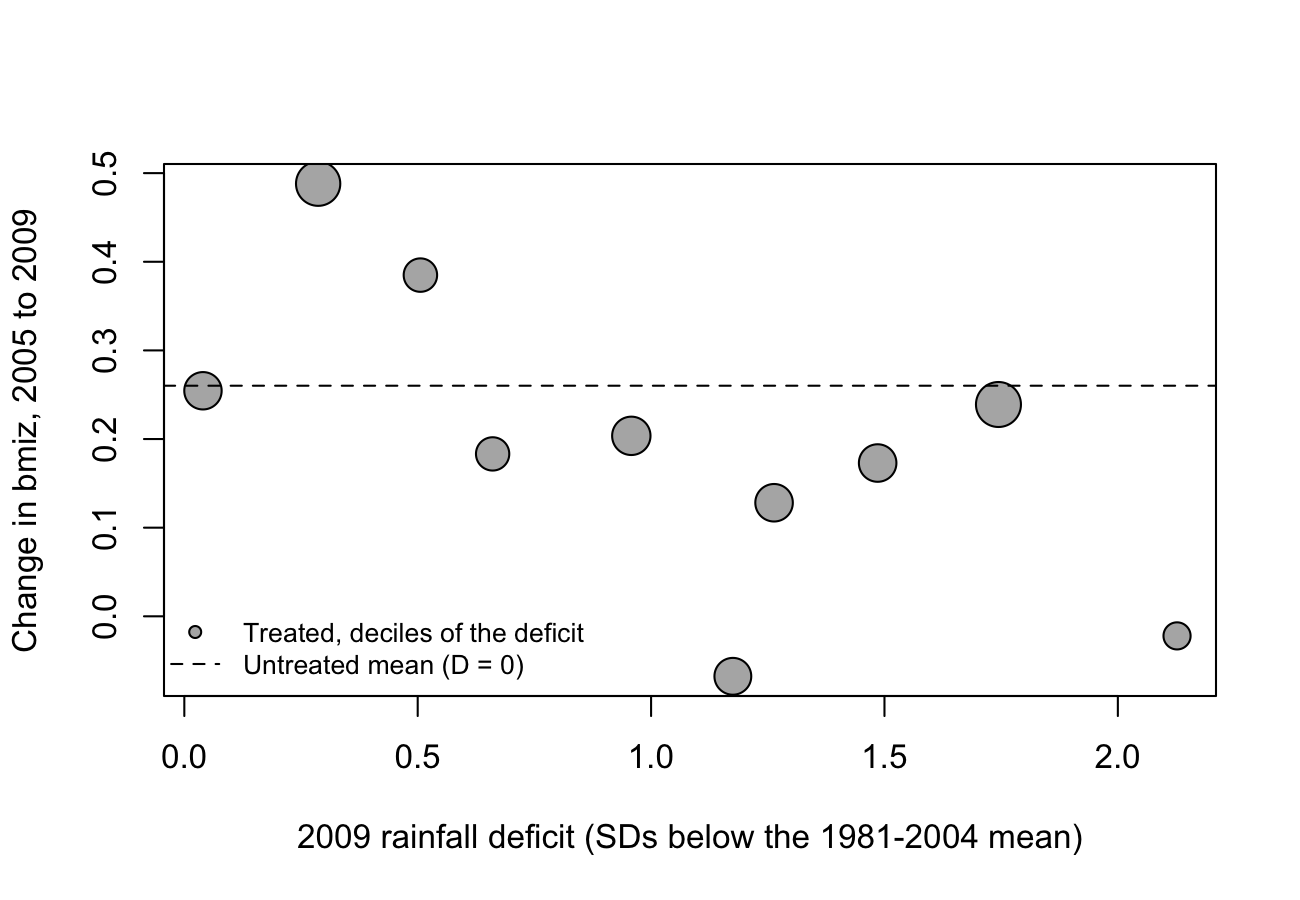
\includegraphics[width=0.8\textwidth]{contdid_binscatter_bmiz.png}
\end{figure}

\begin{figure}[H]
\centering
\caption{Change in Height-for-Age by 2009 Rainfall Deficit, Continuous Dose}
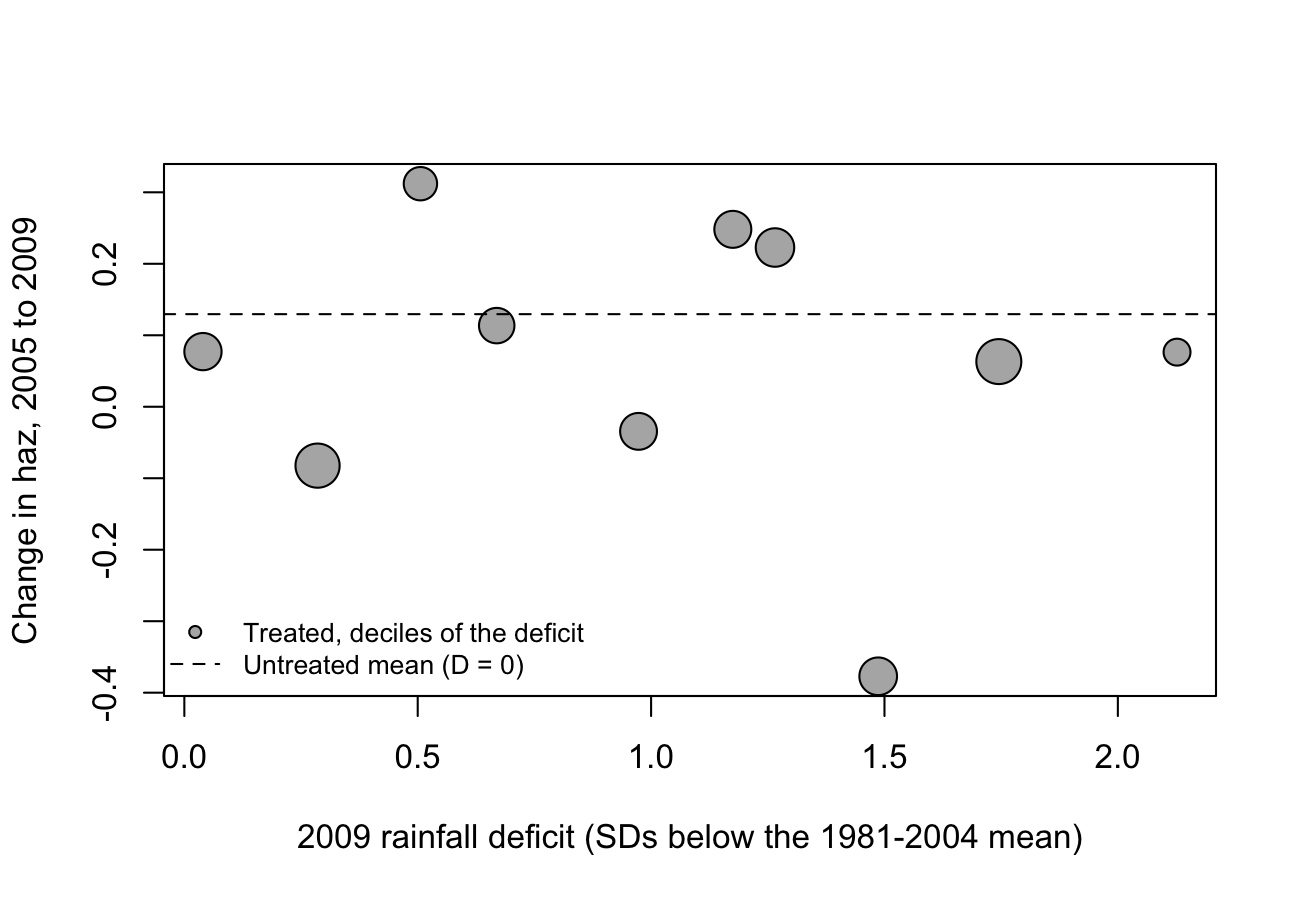
\includegraphics[width=0.8\textwidth]{contdid_binscatter_haz.png}
\end{figure}

\begin{figure}[H]
\centering
\caption{Change in Weight-for-Age by 2009 Rainfall Deficit, Continuous Dose}
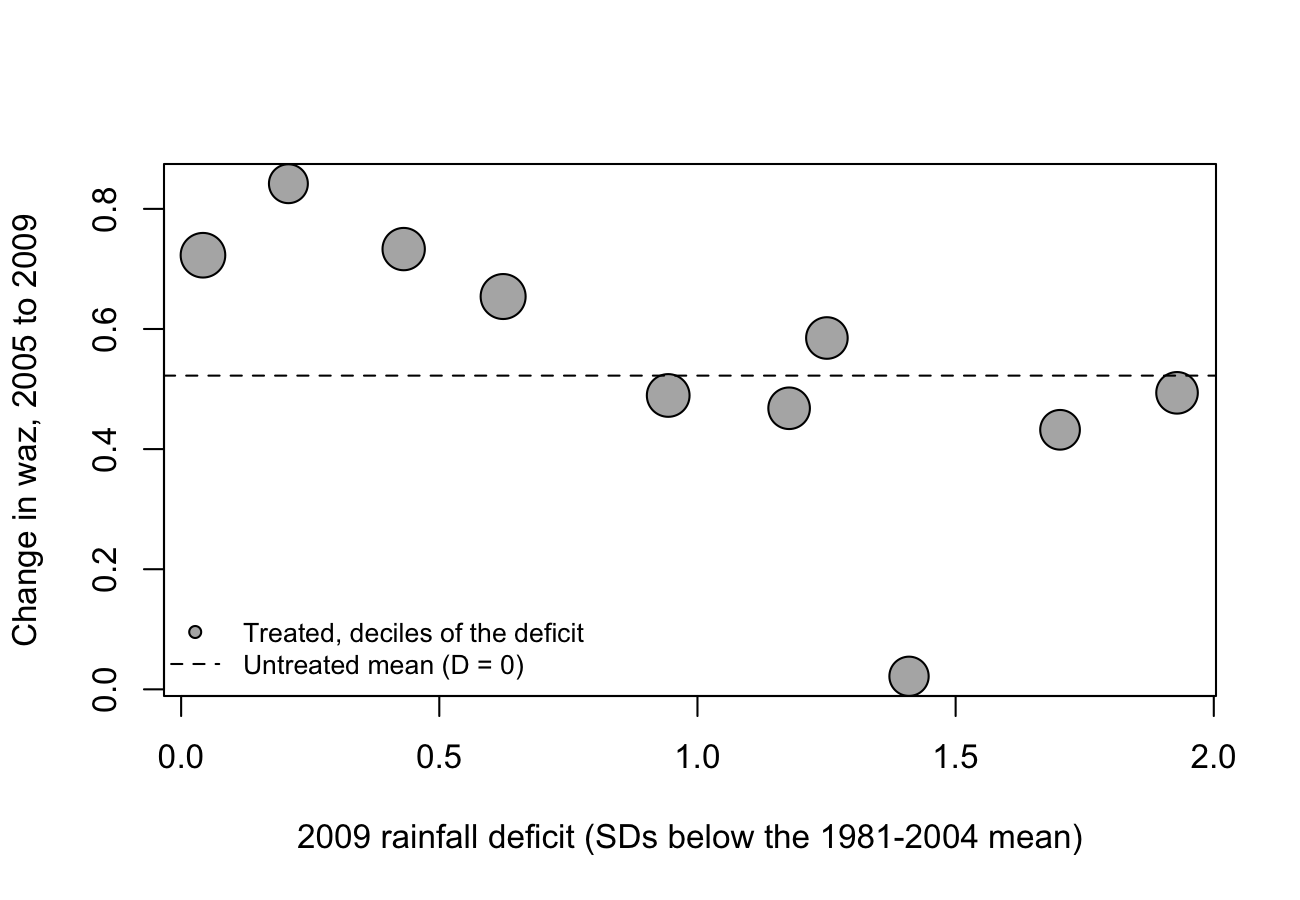
\includegraphics[width=0.8\textwidth]{contdid_binscatter_waz.png}
\end{figure}

\begin{figure}[H]
\centering
\caption{ATT by 2009 Rainfall Deficit, BMI-for-Age, Continuous Dose}
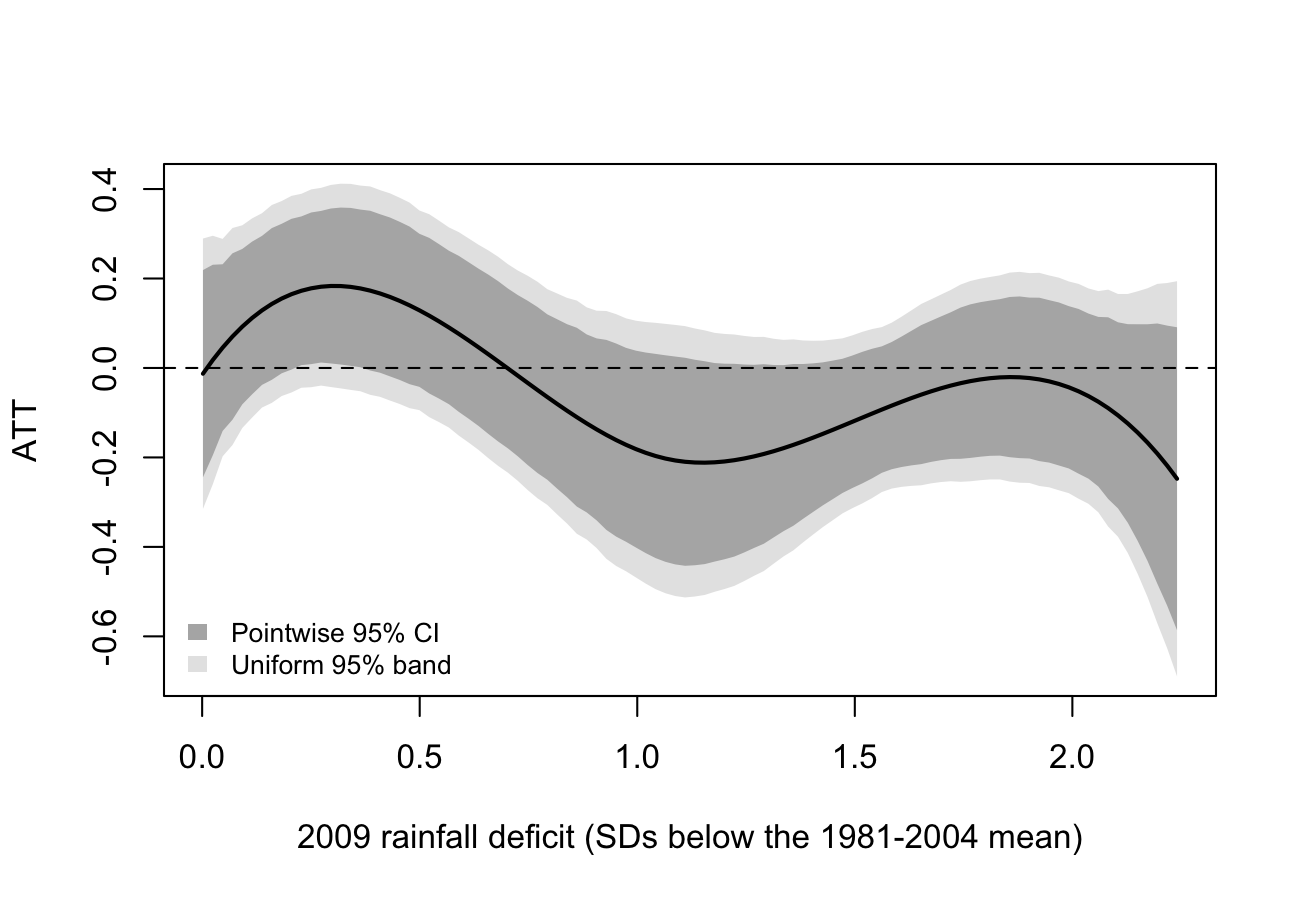
\includegraphics[width=0.8\textwidth]{contdid_att_clustered_bmiz.png}
\end{figure}

\begin{figure}[H]
\centering
\caption{ATT by 2009 Rainfall Deficit, Height-for-Age, Continuous Dose}
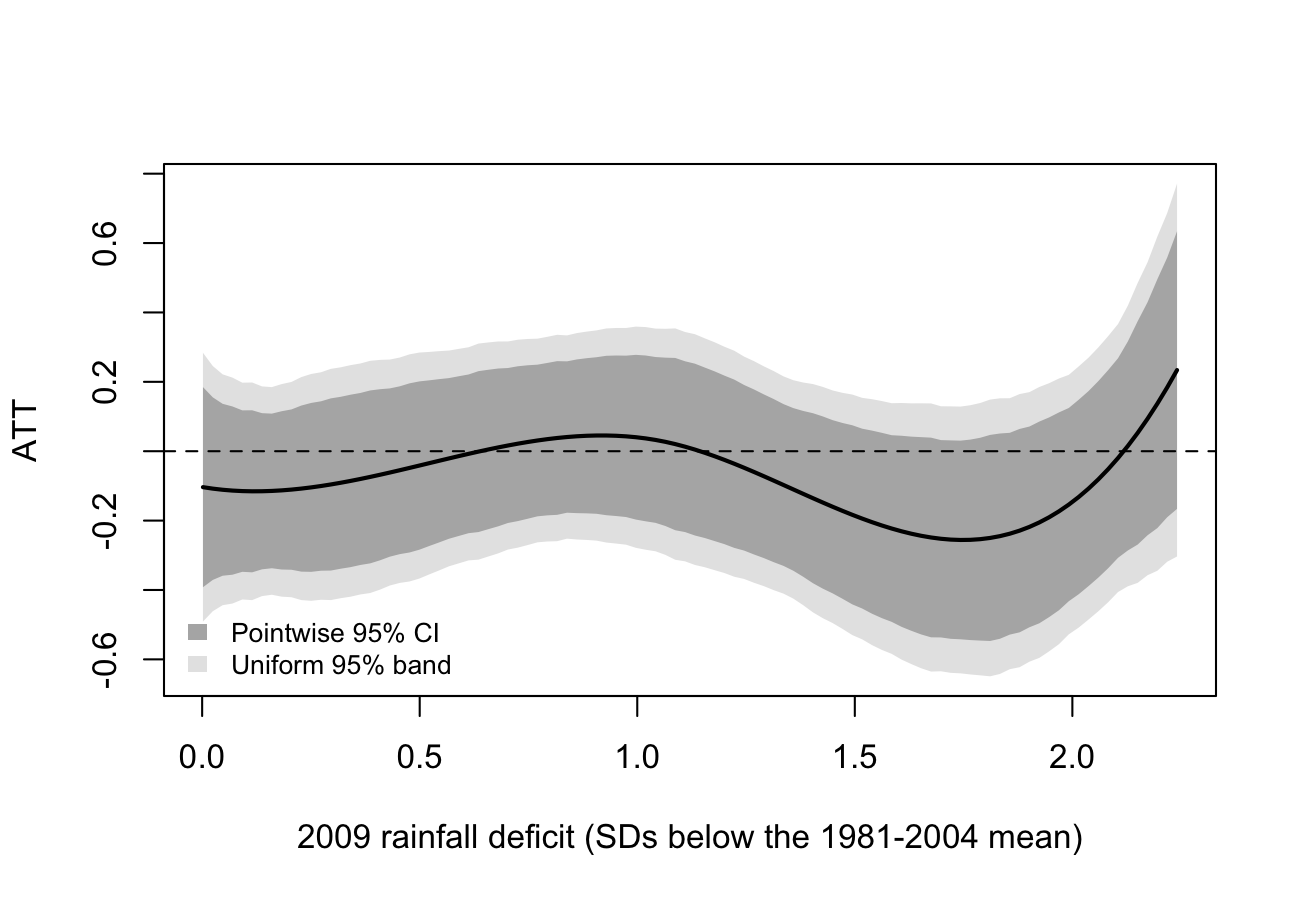
\includegraphics[width=0.8\textwidth]{contdid_att_clustered_haz.png}
\end{figure}

\begin{figure}[H]
\centering
\caption{ATT by 2009 Rainfall Deficit, Weight-for-Age, Continuous Dose}
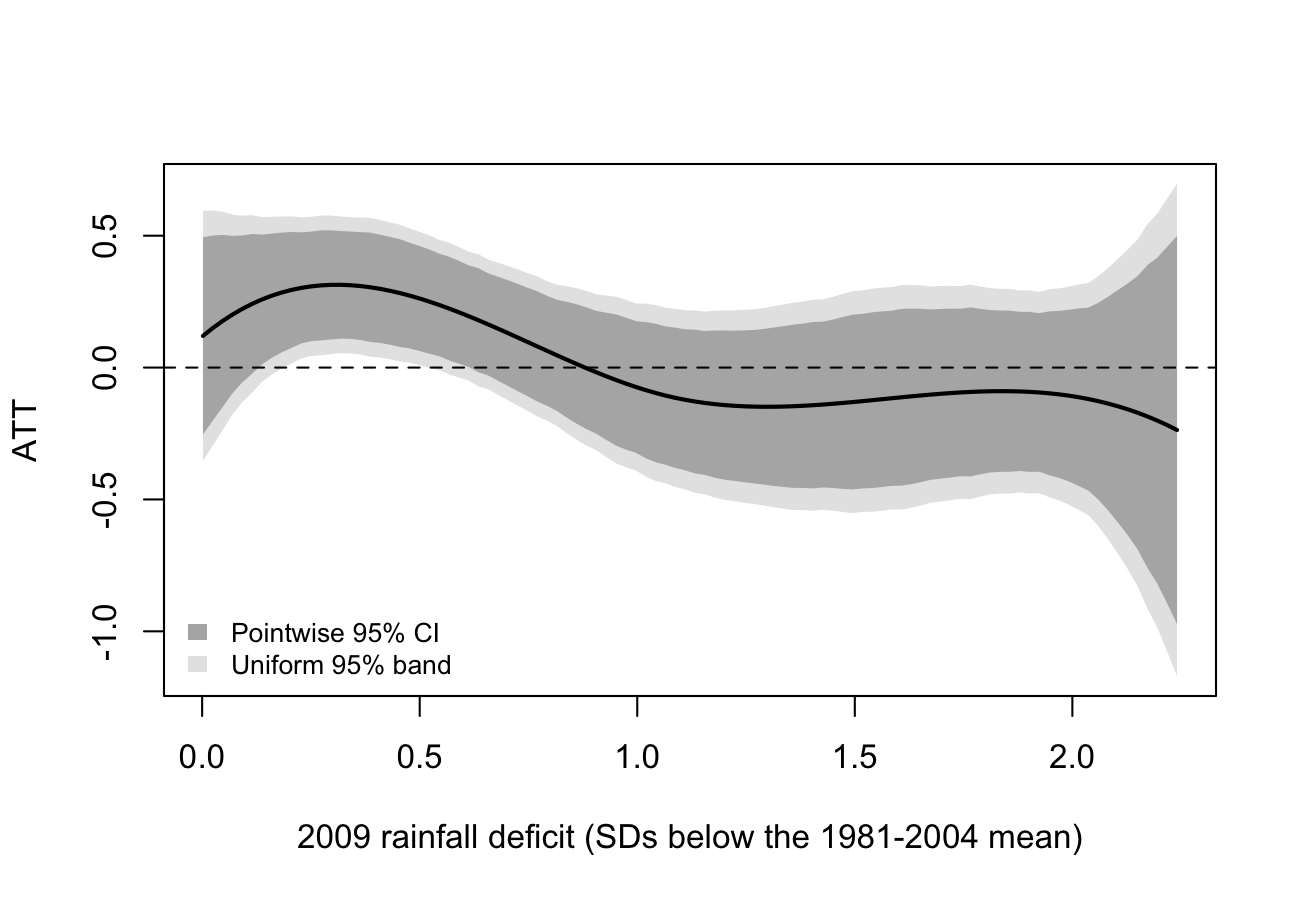
\includegraphics[width=0.8\textwidth]{contdid_att_clustered_waz.png}
\end{figure}

\end{document}
